% Use only LaTeX2e, calling the article.cls class and 12-point type.
% modified by Aaron Clauset (2014) from the scifile.tex file distributed
% by AAAS for articles in Science

\documentclass[12pt]{article}

% Users of the {thebibliography} environment or BibTeX should use the
% scicite.sty package, downloadable from *Science* at
% www.sciencemag.org/about/authors/prep/TeX_help/ .
% This package should properly format in-text
% reference calls and reference-list numbers.

\usepackage{scicite}

% Use times if you have the font installed; otherwise, comment out the
% following line.

\usepackage{times}

% Some standard mathematical notation and figure packages

\usepackage{amsmath}
\usepackage{amsfonts}
\usepackage{amssymb}
\usepackage{graphicx}
\usepackage{float}
\usepackage{multirow}


% The preamble here sets up a lot of new/revised commands and
% environments.  It's annoying, but please do *not* try to strip these
% out into a separate .sty file (which could lead to the loss of some
% information when we convert the file to other formats).  Instead, keep
% them in the preamble of your main LaTeX source file.


\newcommand{\beginsupplement}{%
        \setcounter{table}{0}
        \renewcommand{\thetable}{S\arabic{table}}%
        \setcounter{figure}{0}
        \renewcommand{\thefigure}{S\arabic{figure}}%
     }



% The following parameters seem to provide a reasonable page setup.

\topmargin 0.0cm
\oddsidemargin 0.2cm
\textwidth 16cm 
\textheight 21cm
\footskip 1.0cm


%The next command sets up an environment for the abstract to your paper.

\newenvironment{sciabstract}{%
\begin{quote} \bf}
{\end{quote}}


% If your reference list includes text notes as well as references,
% include the following line; otherwise, leave it commented out. 

%\renewcommand\refname{References and Notes}


% Include your paper's title here

\title{\texttt{efold}: An algorithm to Predict Protein Folding Pathways using Ensemble Modelling and Genomic Variation } 


% Place the author information here.  Please hand-code the contact
% information and notecalls; do *not* use \footnote commands.  Let the
% author contact information appear immediately below the author names
% as shown.  We would also prefer that you don't change the type-size
% settings shown here.

% Authors should be listed in order of contribution to the paper beneath the title on the opening page of the manuscript. Use first name, then middle initial (if any), followed by last name with each name separated by commas. The author list should be one single paragraph with no line breaks.

\author
{David Becerra${}^{1}$ J\'er\^ome Waldisp\"uhl${}^{1\ast}$\\
\\
\normalsize{${}^{1}$School of Computer Science and McGill Centre for Bioinformatics, McGill University,}\\
\normalsize{Montreal, QC, Canada}\\
%\normalsize{${}^{2}$Another Unknown Address, Palookaville, ST 99999, USA}\\
\\
\normalsize{$^\ast$To whom correspondence should be addressed; E-mail:  jeromew@cs.mcgill.ca}
}

% Include the date command, but leave its argument blank.

\date{}



%%%%%%%%%%%%%%%%% END OF PREAMBLE %%%%%%%%%%%%%%%%



\begin{document} 

% Double-space the manuscript.

\baselineskip24pt

% Make the title.

\maketitle 



% Place your abstract within the special {sciabstract} environment.

% The abstract should be a single paragraph, not to exceed 250 words and ideally closer to 200, written in plain language that a general reader can understand. It should include
% An opening sentence that states the question/problem addressed by the research AND
% Enough background content to give context to the study AND
% A brief statement of primary results AND
% A short concluding sentence.
% Do not include citations or undefined abbreviations in the abstract. Any abbreviations that appear in the title should be defined in the abstract.

\begin{sciabstract}
The protein-folding (PF) problem is interested in determining a protein tertiary structure from its amino acid sequence trying to understand the path that leads the folding process.  Understanding the rules that govern the folding of proteins is one of the goals of biophysical studies that are still far from being achieved. High-resolution protein folding dynamics predictions are prohibitive expensive and they are typically produced through custom designed supercomputers and time-consuming molecular dynamics (MD) simulations. For the first time in the literature, we propose a novel methodology (called \texttt{efold}) that unifies the ensemble modeling and the evolutionary based sequence information framework to introduce an efficient (i.e., how well it performs computationally speaking) and effective (i.e., how good its solutions are) ab-initio protein folding method that reflect the ability of proteins to adopt different conformational states in vivo. The proposed method is tested on a benchmark of 125 proteins obtaining excellent results in terms of contact, strand, topology and pathway prediction. \texttt{efold} represents a plausible advance in the PF state of the art through the modeling of the dynamics of protein folding, instead of focusing solely on the native conformation
\end{sciabstract}



% In setting up this template for *Science Advances* papers, both
% the \section* command and the \paragraph* command are used for topical
% divisions.  Which you use will of course depend on the type of paper
% you're writing.  Review Articles tend to have displayed headings, for
% which \section* is more appropriate; Research Articles, when they have
% formal topical divisions at all, tend to signal them with bold text
% that runs into the paragraph, for which \paragraph* is the right
% choice.  Either way, use the asterisk (*) modifier, as shown, to
% suppress numbering.

\section*{Introduction}
% The manuscript should start with a brief introduction that lays out the problem addressed by the research and describes the paper�s importance. The scientific question being investigated should be described in detail. The introduction should provide sufficient background information to make the article understandable to readers in other disciplines, and provide enough context to ensure that the implications of the experimental findings are clear.


The protein folding problem entails advances in understanding the structural basis of protein interactions, as well as in the elucidation, characterization and annotation of protein function. These advances are supported by the understanding of protein post-translational modifications and folding intermediates, the identification of novel protein folds, and potential targets for drug design and treatments for many hereditary diseases \cite{jensen2006interpreting,kihara2002ab}.

The protein folding (PF) problem is interested in determining a protein tertiary structure from its amino acid sequence trying to understand the folding path which leads the folding process. Historically, the PF problem has been split in two related problems, the protein structure prediction problem (PSP) and the pathway prediction problem (PPP). Both problems have been widely acknowledged as open problems, however PSP has received more attention than the PPP problem. Furthermore, the importance of pathway prediction to get valuable insights into the folding process and to guide the search of the conformation space has been neglected. It is clear that the ability to predict folding pathways can greatly enhance structure prediction methods, however, most of the PPP methods starts from a known protein structure (i.e., 3D structure). 

Functional proteins undergo natural selection processes preserving their function hence their structure.  Simultaneously, they must also have good folding dynamic properties that enable them to fold quickly from an unfolded state to the native structure. A functional protein can be characterized by natural selection and/or folding properties. Then, the theory of evolution and the laws of physics are the principles on which the techniques of protein structure prediction are based.  Comparative and fold recognition methods for protein structure prediction belong to the first characterization and they rely on the similarity between a target protein and a set of known protein structures at the fold level. By contrast, ab-initio methods focus on the second aspect and predict protein structure based on laws of physics, biology and chemistry without considering any related structure as template.

A number of computational and experimental techniques for protein folding pathway prediction already exists in the literature, but most of them are limited by the required amount of time and resources, or the restrictive assumptions imposed during the modeling process. State of the art methods are currently unable to compute, and even approximate, the complete 3D conformational landscape for all protein targets. Then, there is a tangible need in the structural biology research field to develop efficient and effective protein folding methods. The ensemble modeling and evolutionary information content-based methods belong to a newer and promising group of approaches that aims to offer a better trade-off between efficiency and accuracy for predicting structures and folding pathways.

Ensemble modeling methods employ a coarse-grained structural model that enables us to efficiently compute a complete conformational landscape and apply statistical mechanics techniques. Many current obstacles presented in the protein folding problem have been already addressed by research in RNA.  Specifically, the development of structural ensemble prediction algorithms have allowed the accurate computation of RNA secondary structure energy landscapes and sample structures from sequence information alone \cite{ding2003statistical,mccaskill2004equilibrium}.  Although, those approaches can not directly be mapped to proteins, they have been an excellent starting point to model more accurate and complex scenarios. With respect to the protein structure scheme,  we have already introduced a structural ensemble predictor for transmembrane $\beta$-barrel (TMB) proteins \cite{waldispuhl2008modeling} continuing earlier work on molecular structure modelling \cite{waldispuhl2006predicting,waldispuhl2005modeling}. We also introduced a method for modelling the folding process of large $\beta$-sheet proteins using sequence data alone \cite{shenker2011efficient}.

The prediction of 3D protein structures using evolutionary sequence information is a novel statistical approach in which evolutionary constraints are inferred from a set of sequences belonging to an iso-structural protein family \cite{marks2011protein}. These methods use the information gleaned from statistical analysis of multiple sequence alignments to reduce the space of 3D protein conformation where the 'native' structure can be identified. The evolutionary sequence variation methods have been criticized for their little use in protein structure prediction due to their low accuracy. However, their usefulness debate has received new momentum with the rise of novel and accurate approaches that allows the systematic application to 3D structure prediction studies.

In this work, we introduce \texttt{efold}, a new protein folding pathway prediction framework that combines ensemble-modeling techniques with evolutionary sequence information methods. efold is a general framework that enables efficient simultaneous prediction of the protein folding mechanism and structure using only the primary sequence as input. efold also expands our previous protein folding prediction frameworks in several directions while keeping its low CPU-time requirements. First \texttt{efold}  models  $\alpha$-helices and multiple $\beta$-sheets. Next, \texttt{efold}  algorithm applies memoization techniques and computes the conformational landscape of all $\beta$-sheet topology i.e. number of $\beta$-strand with their relative positions at once, hence avoiding redundant calculations and decreasing the computational complexity. Finally, to the best of our knowledge, for the first time the residue contact information is integrated in the Boltzmann sampling process performed by ensemble methods to predict protein pathways. The proposed method is tested on a benchmark of 125 proteins obtaining excellent results in terms of contact, strand, topology and pathway prediction.


\section*{Results}
% The results should describe the experiments performed and the findings observed. The results section should be divided into subsections to delineate different experimental themes. Subheadings should either be all phrases or all complete sentences. All data must be shown either in the main text or in the Supplementary Materials.
% 
% All data should be presented in the Results. No data should be presented for the first time in the Discussion. Data (such as from Western blots) should be appropriately quantified.
% Subheadings must be either all complete sentences or all phrases. They should be brief, ideally less than 10 words. Subheadings should not end in a period. Your paper may have as many subheadings as are necessary.
% Figures and tables must be called out in numerical order. For example, the first mention of any panel of Fig. 3 cannot precede the first mention of all panels of Fig. 2. The supplementary figures (for example, fig. S1) and tables (table S1) must also be called out in numerical order.
% Display equations (set on their own line) can be included. Do not use the native Word 2007, 2008, 2010, or 2011 equation editor. This can in produce inaccurate MathML, the online markup language we use, which may result in display errors. Instead, use the legacy equation editor in Word (Insert menu; select insert object; select word equation) or use MathType (recommended). If you enter equations in simple LaTeX, check that they will convert accurately (Word 2007 and higher can convert simple LaTeX equations). Display equations should be numbered at the right�(1), (2), etc.
% The same guidelines apply to mathematical expressions within a sentence of text; however, MathType (or the equivalent) should be used within text only when the desired result cannot be achieved using ordinary Word characters. Reserve MathType for when its use is unavoidable�for example, characters with overbars or carets, with stacked superscripts and subscripts, or within square root symbols.
% All data must be shown; references to �unpublished results� or �data not shown� are not permitted.

In order to understand the performance of the proposed method, experiments were performed to study the modeling ensemble (protein structure prediction) and modeling folding phases (protein pathway prediction). \texttt{efold} is run having as input only the amino-acid sequence and a set of parameters. Then, the algorithm runs until all the folding pathways and structures have been computed. Based on the experimental framework and user experiences with our previous techniques, we have fixed the limits of our algorithm to predict the folding pathways for small proteins (less than 200 amino acids), and to model proteins with up to 7 different $\beta$-sheet strands. It is important to stress that when comparing our results with experimental and computational experiments, the numeration used for the strands follows the numeration proposed in our methodology.  

Even if \texttt{efold} is not an algorithm developed to predict residue-residue contacts, we evaluated the prediction capabilities of \texttt{efold} to recognize contacts involved in secondary structures. Then, we tested the proposed algorithm using the complete protein benchmark and compared the performance of \texttt{efold} with the predictions performed by EVfold and by our previous algorithm tfolder. We are also interested in study the \texttt{efold} capabilities to predict contacts involved in secondary structures. The prediction of those contacts is studied following the same methodology than normal residue-residue contacts. A pair of residues is considered to be part of $\beta$-strand interactions if the predicted residues are contacts and those contacts are observed to be involved in a $\beta$-sheet interaction in its corresponding PDB file. The results for the contacts and strand prediction are discussed in the Section \ref{sec:contact_and_strand_prediction}.

The experiments reported in Section \ref{sec:topology_prediction} quantify the ability of \texttt{efold} to correctly rank the admissible $\beta$-sheet topologies. \texttt{efold} performs the generation of all the admissible $\beta$-sheet topologies and the computation of the Boltzmann partition function over those topologies. Next, \texttt{efold} ranks those topologies based on their energy states and it clusters the top low-energy states to predict the folding dynamics. Then, for each protein in the benchmark, we are interested in quantify the position of the topology reported by the corresponding PDB file in the rank computed by \texttt{efold}.

To study the efficacy of our technique for predicting protein-folding pathways, we studied the folding landscape of proteins for which their pathways have been elucidated through many experimental studies and/or MD. A graph for a specific folding pathway was constructed by considering all pairs of clusters computed during the modeling ensemble phase. If the minimum distance between two clusters was less than the transition threshold, we considered that there was exchange between the two states. The results of this pathway prediction procedure are discussed in Section \ref{sec:pathway_prediction}.

Understanding the rules that govern the folding of proteins is one of the goals of biophysical studies that is still far from being achieved. Two different strategies have been shown suitable in biophysical studies to extract general rules from the protein folding process. The first approach works by comparing the mechanisms of proteins sharing the same overall fold but different sequence, i.e., members of the same protein family. The second strategy analyzes proteins with a high degree of sequence identity, but different 3D structure. The results of our experiments based on the first technique are reported in Section \ref{sec:different_structure}. On the other hand, results based on the first strategy are reported in Section \ref{sec:different_sequence}.


\subsection{Contact and Strand Prediction}

\label{sec:contact_and_strand_prediction}


The first experiment quantify the ability of  \texttt{efold} to predict protein topologies through the prediction of  residue-residue contacts. We sample 150 configurations for each protein of the benchmark, and use these ensembles to compute a stochastic contact map. The contact map represents the probability of observing a given contact. Contacts are defined as all $C_\alpha$ atoms less than $8\AA$ apart in the PDB file. The precision, sensitivity and F-measure were the chosen measures to assess the effectiveness of the method. These metrics are evaluated for all types of contacts (short, medium, and long-range). Particularly, an evaluation is performed when predicted contacts are within exact or $\pm2$ residues of an observed contact, and are more than 0, 12 and 24 residues apart.

Figure \ref{fig:boxplots} (column \textit{Contact prediction}) reports, through box plots, the best results of the experiments for the complete set of proteins (row \textit{Complete}) and the set divided by the number of strands in the tested proteins (see Figure TBD). It is important to notice that the proposed method predicts residue contacts with an excellent precision for $\pm2$ for all contact separations in the complete benchmark. The precision for exact prediction (i.e., columns $\pm0$) is also high and it averages around $50\%$ for the short and medium contacts and around $33\%$ for long-range contacts. This result is significant given that critical protein folding steps can involve both short range and long-range $\beta$-sheet contacts and that the precision assessed state-of-the-art algorithms in contact prediction for proteins without homology-based templates averages around 20\% \cite{monastyrskyy2014evaluation}. The recall obtained by \texttt{efold} average around $10\%$ and $30\%$ for contacts $\pm 0$ and $\pm 2$, respectively. This results is low as expected given that \texttt{efold} does not aim the prediction of all residue contacts, but those involved in secondary structures. 

Comparing the predicted residue contacts between \texttt{efold} and our previous model tfolder for the Protein G, it is worth noticed in Table \ref{tb:comparison} that \texttt{efold} shows a better predicted accuracy than the tfolder algorithm. Furthermore, the proposed method performed better than tFolder in all the ranges except for the exact observed contacts studied 24 residues apart. The proposed approach not only kept sensitive to the distance of contact separation, but it increased the precision and sensitivity of the ensemble method. 

\texttt{efold} is also compared with evfold to measure at which extent \texttt{efold} improve the residue contact predictions used as input in our method. Particularly, the $500$ best ranked evolutionary inferred contacts (i.e., EICs) computed by evfold are used as input in \texttt{efold} (see section Methodology for more details).  Figure \ref{fig:boxplotsevfold} (column \textit{Contact prediction}) reports, through box plots, the results of the experiments for the complete set of proteins. The recall of evfold for $\pm2$ averages around $40\%$ for all the range of contacts. Then, evfold gets a better coverage than \texttt{efold} given that, unlike \texttt{efold}, evfold does not focus only in contacts involved in secondary structures. Regarding the precision of the evfold results, its low performance can be explained by the dependence of evfold on the depth of the target alignments (See supplementary Table 1 for a complete list of the size of MSAs).  Figure \ref{fig:boxplotsevfold} shows that the methodology implemented by \texttt{efold} improved the initial contact predictions performed by evfold. 

Figure \ref{fig:boxplots} (column \textit{Strand prediction}) reports, through box plots, the best results of the experiments for contact prediction of residue-residue contacts involved in $\beta$-sheet structures. The results are spliced in rows showing the complete set of proteins (row \textit{Complete}) and the set divided by the number of strands in the tested proteins. It is important to notice that the F-measure values for $\pm2$ for all contact separations in the complete benchmark is higher than $60\%$. This result corresponds to a very good performance of the method in terms of its accuracy and sensitivity. Furthermore, it confirms \texttt{efold} as a very good predictor of contacts involved in secondary structures. Regarding the exact prediction (i.e., columns  $\pm0$), the precision decreases for long range contacts. Particularly, it  goes from a precision around $30\%$ for the complete set of contacts to a precision around $20\%$ in long range contacts. The best and worst performance of \texttt{efold} can be recognized in proteins with three and two strands, respectively. It is important to stress that in \texttt{efold} there is not a big difference between the precision and sensitivity values for strand predictions, given that \texttt{efold} focuses on predicting contacts involved only in secondary structures.

Figure \ref{fig:boxplotsevfold} (column \textit{Strand prediction}) reports, through box plots, the results of the experiments performed by evfold for the complete set of proteins. It is important to notice that these results are more homogeneous than the results obtained in the contact prediction experiment. Moreover, there is not a big difference in the behaviour of the precision and recall measures, as noted in the contact prediction column. There is not a big difference either between the contacts $\pm 0$ and $\pm 2$ for all the contact ranges. The average of all the evaluation measures for an exact prediction ($\pm 0$), for the strand prediction experiment, fall in the same range (i.e., below a $10\%$) than its contact prediction counterpart.  Then, it gives the insight that most of the contacts predicted by evfold are involved in secondary structures. On the other hand, there is a clear decrease of the recall of the strand prediction with respect to the contact prediction, suggesting that for ($\pm 2$) predictions, evfold reports a greater quantity of contacts not involved in secondary structure than the exact predictions ($\pm 0$).  The prediction values for evfold are much lower than the values of \texttt{efold}, showing that the methodology implemented by \texttt{efold} improved the initial contact predictions performed by evfold regarding contact and strand predictions. 

\subsection{Protein Topologies Prediction}

\label{sec:topology_prediction}

Figure \ref{fig:boxplots} (column \textit{Rank}) reports, through box plots, the position occupied by the PDB topologies in the ranking computed by \texttt{efold}. Particularly, for each protein composed by $L$ strands, the position with respect to the top percentage when considering all the topologies with $L$ strands (column \textit{All}) and the attainable topologies given a common parent with $L-1$ strands (column \textit{P}) are computed. It is important to stress that the likelihood of a specific topology to be chosen by \texttt{efold} to create clusters of low-energy states (used to predict the folding dynamics) increases as the topology move to the head of the ranking-list.

Figure \ref{fig:boxplots} (column \textit{Rank}) shows that, in average, the proposed approach ranks the target topologies (i.e., the topologies reported in the PDB) in the top $2\%$ for the categories \textit{All} and \textit{P}. The best performance is computed for proteins of two and five strands. On the other hand, proteins of three strands compute the worst performances. \texttt{efold} performs better when the ranking is computed for all the the admissible $\beta$-sheet topologies (column \textit{All}), than when compared with a subset (column \textit{P}). Figure \ref{fig:boxplots} (column \textit{Rank}) shows excellent discrimination power of \texttt{efold} to separate conformational transitions that are critical to folding from those transitions that could simply result from minor structural fluctuations. In other words, \texttt{efold} allows the sampling of accurate conformations and it also score accurately those models more favourably from other decoys.   

\subsection{Protein Pathway Prediction}

\label{sec:pathway_prediction}

To measure at what extent the predictions of evfold influenced the\texttt{efold}'s predictions, runs with different influence of evfold parameters where computed. Specifically, the parameter $\gamma$ (see equation TBD) was set from a value of $0$ (i.e., The evfold predictions has not inference in the computation of the state's energy) to a value of $1$ (i.e., The computation of the state's energy is based completely on the evfold predictions) through adding $0.1$ to the parameter $\gamma$. Five independent runs were computed for each experiment. Then, a total of $50$ simulations were computed for each of the following experiments. 

\subsubsection{Protein G}

Figure \ref{fig:Pathways_1EM7} reports a graph that represents the predicted folding transitions for protein G. The folding landscape and pathway of the peptide were reconstructed following the proposed methodology (see Section Methods). Inspection of this figure reveals that the folding intermediates are consisted with previous literature reports. Specifically, it is consistent with the work reported by (\cite{blanco1994short,kuszewski2008fast}), with respect to the early formation of the second hairpin ($\beta3 - ~turn -\beta4$) and its fundamental role in the folding process. Additionally, this second hairpin centers around known nucleation points W43, Y50, F54 that are strongly stabilized by three hydrophobic residues W43, Y45 , F52 (\cite{hubner2004commitment}) (See figure TBD). Our results also shows an early formation of the first hairpin ($\beta1 - ~turn -\beta2$)) and folding pathways were observed passing through the intermediate $\beta1-~\beta4$ sheet. This agrees with studies \cite{shimada2002ensemble, hubner2004commitment} were it has been shown that proteinG folds through three pathways, all of which pass through an intermediate, to a single transition state. The three intermediates feature a near-native helix along with one go the three states determined by our simulations. Four folding pathways were observed in the simulations. Particularly, $80\%$ of folded runs passed through a $helix - hairpin 1$ complex (red pathway in Figure \ref{fig:Pathways_1EM7}), $16\%$ of the runs have a $helix - hairpin2$ complex and the $64\%$ a $\beta1-\beta4$ sheet complex. These pathways agrees with those found in \cite{shimada2002ensemble}. Given the complexity of the chain topology, folding and intermediate states, we can expect a statistical distribution of topologically allowed pathways for assembling the tertiary fold as the ones found by our simulations.

Comparing the predicted folding pathways between \texttt{efold} and our previous model tfolder (See Supplementary Figure TBD), it is worth noticed that both models were able to predict the reported pathway for the tested protein; however, the probability of the experimental folding pathway is higher for \texttt{efold} than tfolder. The previous fact means that \texttt{efold} was more likely to correctly predict the observed folding pathway than its counterpart. Additionally, it is clear that \texttt{efold} was able to narrow the number of generated and predicted templates. There are two main factors that could help \texttt{efold} to got this performance with respect to tfolder. $i)$ The penalization term used in \texttt{efold}, which penalizes the protein conformations that superimpose a $\beta-strand$ where an $\alpha-helix$ structure was predicted, allowed the model to narrow the search around conformational transitions that are critical to folding. $ii)$ The hierarchical assembly folding model used in \texttt{efold} could represent a step-wise mechanism to narrow the conformation search through the correct prediction of the initial stages of protein folding process.

\subsection{Ubiquitin}

Figure \ref{fig:Pathways_1UBQ} reports a graph representing the predicted folding transitions for ubiquitin protein. Inspection of this figure reveals that our simulations are in agreement with a view of ubiquitin folding suggested from previous experimental results and in-silico simulations. Particularly, our simulations give a special importance to a topology encompassing the $\beta1$ and $\beta2$ strand. This topology has been described to participate in a polarized and well-defined transition state ensemble \cite{piana2013atomic,sosnick2004differences,went2005ubiquitin}. Regions of the local $\beta1$-$\beta2$ hairpin populate native geometries, then this secondary structure can be stabilized by tertiary interactions between the $\alpha$-helix and the $\beta1$-$\beta2$ sheet. 

Computational analysis of experimental $\phi$-values suggested that strands $\beta3$ and $\beta5$ might be formed adopting a native-like topology in the TSE \cite{varnai2008determination}. Furthermore, $\psi$ analysis suggested that ubiquitin folds through a much more organized TS ensemble with a common nucleus consisting of a partially formed four-stranded sheet network ($\beta1~-~\beta2~-~\beta5~-~\beta3$). Then, in the ubiquitin folding pathway, regions of the local $\beta1$-$\beta2$ hairpin populate native geometries. Next, strand $\beta5$ joins the nascent hairpin-helix nucleus. Finally, the more distal strand $\beta3$ is joined to the core structure cite{krantz2004discerning}. Our simulations show an important role of the topology $\beta3~-~\beta5$ when combining with the topology $\beta1$-$\beta2$. Particularly, it can be noted that the topology  ($\beta2~-~\beta1~-~\beta5~-~\beta3$) is the most populated edge in the graph. This topology receives the flow containing most of the in-coming paths. Furthermore, this topology represents also the edge with more connections with the edge representing the native topology (i.e., ($\beta4~-~\beta3~-~\beta5~-~\beta1~-~\beta2$)).  The different paths coming into the topology $\beta2~-~\beta1~-~\beta5~-~\beta3$ can represent the heterogeneity predicted for the transition state structure. The routes that stem from the core nucleus represent the heterogeneity of the transition state. The TS ensemble can contains subpopulations with additional structure formation.Particularly, this topology contains all the obligatory elements, but the nucleus of the TS structure can spread in different directions, adding more $\beta1~-~\beta2$ or more $\beta3~-~\beta5$ structures. 

\subsection{SH3 domain}

Figure \ref{fig:Pathways_SH3} reports a graph that represents the predicted folding transitions for proteins having the SH3 domain. Specifically, the proteins 1OOT, 1I0C, 1NEG and 2HDA were used to simulate the transitions from a random coil to the native state of proteins having this domain. Through the analysis of this figure, it is clear that the pathway crossing the four stranded $\beta-$sheet $\beta1-\beta2-\beta3-\beta4$ (yellow path in Figure \ref{fig:Pathways_SH3}) was present in $80\%$ of the simulations. Then, the studied SH3 domains agree in the formation of the $\beta1-\beta2$, $\beta2-\beta3$, and $\beta3-\beta4$ motifs.  Previous findings \cite{neudecker2012structure} suggested that this topology constitutes a metastable folding intermediate. This intermediate has been shown to be highly aggregation prone, as it exposes Strand $\beta1$. Then, the formation of native strand $\beta5$ (i.e., last folding step in the path) is critical in preventing aggregation during folding, where the native state is protected from aggregation, whereas the intermediate is highly aggregation prone.

Three of the predicted pathways cross through the $strand2 ~ strand3 ~ strand4$ topology. Experimental results indicate that the second, third, and the fourth $\beta$-strands are the most ordered regions of the TSE. This structure is common to all the domains simulated in our experiments and it represents  the central (and hydrophobic) sheet $\beta2 ~ \beta3 ~ \beta4$. From that topology, the paths branch in three different pathways (i.e., the red, purple and yellow paths in Figure \ref{fig:Pathways_SH3}). These path counts for the most probable paths and end the folding building the second sheet (a less structured topology) with two terminal strands ($strand1 and strand5$). 

It is important to stress that this protein does not contain $\alpha$-helix motifs, showing that the evolutionary inference contact is able to correctly model $\beta$-strands motifs in the absent of other secondary structures.  Then, the use of evolutionary information is applied not only as a constraint factor, but as a complementary module to the ensemble modelling procedure.  


Figure TBD shows how the probability of observing any of the reachable states changes over time. Given the expected low probability of high size permutations, these values have been normalized for each size of pairing interactions. Interestingly, there are many interactions of three pairings (i.e., four $\beta$-strands), which agrees with previous findings about that four stranded $\beta$-sheet constitutes a metastable folding intermediate (\cite{neudecker2012structure}). 


\subsection{Sequence vs Structure}

\label{sec:different_sequence}

An novel engineering approach allowed the obtention of set of proteins with high sequence identity but different structure and function \cite{giri2012folding, alexander2007design,he2008nmr}. Particularly, the sequences of two domains from streptococcal protein G were subjected to an iterative design of heteromorphic pairs. Then, two different wild-type protein domains, called $G_{A}$ and $G_{B}$ showing an increasing degree of sequence identity (starting from $1\%$ to $95\%$) have been created.  $G_{A}$ displays a three-helix bundle fold, and $G_{B}$ displays a $\alpha + \beta$ proteinG fold. Table \ref{tb:identity} shows the percentage identity between the different variants of the wild-type proteins and proteinG.  These set of proteins represent a great opportunity to elucidate relationships and dependency between \texttt{efold}, sequence information and folding mechanisms.

Figure \ref{fig:Pathways_1EM7B} reports a graph that represents the predicted folding transitions for the variants and wild type proteins for the GB folds. Special interest is given to the GB folds given than \texttt{efold} is an algorithm for modelling the folding process of large $\beta$-sheet proteins, such as the $\alpha + \beta$ ubiquitin-like fold reported by the GB folds. From figure \ref{fig:Pathways_1EM7B} it is clear that four main set of pathways can be obtained from the simulations. Specifically, the first group is constituted by the variants $G_{B88}$ and $G_{B95}$, the variants $G_{B77}$, $G_{B33}$ and $G_{B1}$ composed the second, third and fourth groups, respectively. Comparing those sets, it is important to stress that the blue path is the most probable path in all the sets. These pathways correspond to the early formation of the second hairpin ($\beta3 - ~turn -\beta4$) and the first hairpin ($\beta1 - ~turn -\beta2$) followed by the formation of the $\beta1-~\beta4$ sheet. The red pathway is also highly present in our simulations. This pathway favours the early formation of the first hairpin followed by the formation of the sheet and second hairpin. These behaviours agree with the folding pathways attributed to a ProteinG like fold. Beside the common folding paths, our simulations exhibit distinct folding routes for the protein G variants. Particularly, the variants $G_{B95}$ and $G_{B}$ exhibit an  path based on an early formation of the second hairpin followed by a $\beta1-~\beta4$ sheet formation (orange path in Figure \ref{fig:Pathways_1EM7B}) that is not present in the other variants. Additionally. the wild type $G_{B95}$ does not show the path involving an early formation of the $\beta1-~\beta4$ sheet. The previous simulations agree with the evidence that proteinG variants exhibit distinct folding routes, where the main difference between them is a different order of formation of the $\beta$-strands \cite{lindorff2011fast}.

This experiment is also useful to analyze the sensitivity of \texttt{efold} to changes in the amino-acid sequence. In particular, it is clear that \texttt{efold} is sensitive enough to preserve the prediction of pathways for proteins that diverge in amino-acid sequence, but that contains similar folding pathways. In a similar way, \texttt{efold} was able to diverge the prediction of folding pathways that present a high sequence identity, but different folding pathways. Particularly, when comparing the ranking (as explained in the Section \ref{sec:topology_prediction}) between the variants of GA folds versus the variants of GB folds, the predictions of the GB folds, as a ProteinG fold-like, outperform the predictions of the GA counterparts. In other words, \texttt{efold} was able to predict with high accuracy the GB folds as containing a ProteinG fold-like topology; meanwhile \texttt{efold} predicted the GA folds as topologies with a low probability to belong to a ProteinG topology. It is important to stress that this divergent predictions were obtained on proteins with a high sequence identity, but different 3D structures. 

\subsection{Pfam families}

\label{sec:different_structure}

Experimental studies suggest that the native topology of a protein plays a key role in determining its folding pathway. These studies usually compare proteins that differ in sequence but share the same overall fold to identify relationships between sequence information and folding mechanism. As a result, the folding mechanisms of proteins belonging to a same protein family have been reported as conserved \cite{travaglini2009folding, zarrine2005family}. In this section, we analyzed the results of comparing folding processes of different members of four protein families. Particularly, the Pfam families PF00014, PF00018, PF00240,  and PF01423 are studied.  

\subsubsection{PF00014}

Figure \ref{fig:Pathways_PF00014} reports a graph that represents the predicted folding transitions for proteins belonging to the Pfam family PF00014. Specifically, the proteins 1D0D, 1BUN, 1BIK and 5PTI were used to simulate the transitions from a random coil to the native state of proteins having this domain. Through the analysis of this figure, it is clear that there are two pathways that are present in all our simulations. The final topologies are represented by $1A2N3A4$ and $2A1A3$ arrangements. These topologies are attributed to the proteins 1BIK and 5PTI, respectively.  The topology $1A2$ is traversed for all our simulations and it is present in all our simulations.
 
The folding pathways of disulfide proteins vary substantially \cite{arolas2006folding}.  Particularly, it has been shown that with two structurally homologous kunitz-type protease inhibitors, bovine pancreatic trypsin inhibitor and tick anticoagulant peptide, there is a heterogeneity of folding intermediates and folding kinetics \cite{chang2011distinct}. The simulated proteins represent three different kunitz-type protease inhibitors. Specifically, two proteins (1D0D, 5PTI,) represent bovine pancreatic trypsin inhibitors (BPTI), 1BUN represent a serine protease inhibitor homolog beta-bungarotoxin B2 chain and 1BIK represents a AMBP protein.  The proteins BPTI simulated in our experiments show a unique folding pathway with an early formation its secondary structures. This result agrees with experimental results that suggest for BPTI, the stable subdomain structures dictate the formation of native-like intermediates and limit the heterogeneity of folding intermediates \cite{chelvanayagam1993prediction}.

\subsubsection{PF00018}

The results have been already analyzed in the section SH3 domain.

\subsubsection{PF00240}

Figure \ref{fig:Pathways_PF00240} reports a graph that represents the predicted folding transitions for proteins belonging to the Pfam family PF00240. Specifically, the proteins 1CMX, 1EUV and 1UBQ were used to simulate the transitions from a random coil to the native state of proteins having this domain. Through the analysis of this figure, it is clear that the topology $\beta2~-~\beta1~-~\beta4~-~\beta3$ is the conserved topology for the family. This topology corresponds to the organized TS ensemble that consist of a four-stranded sheet network (i.e,. $\beta2~-~\beta1~-~\beta5~-~\beta3$) in the folding pathway of the ubiquitin protein. 
The different paths that converge to the conserved structure can represent the different proportions of the four properly aligned strands that compose the $\beta$-sheet network. The two most populated paths (green (71\%) and red (60\%)) cross through the topology $\beta2~-~\beta1~-~\beta4$, showing concordance with the ubiquitin folding suggested from experiments. The strand $\beta4$ is present in all the paths that convert to the final topology. This strand is the central strand and a critical structural component in the ubiquitin topology.

The topology  $\beta2~-~\beta1~-~\beta4~-~\beta3$ is topographically related to the structure of ProteinG in that the order, positions and stretches of secondary structures are identical. This fact is important given that  it has been shown that this fold is present in the ubiquitin family an in other proteins with biologically distinct functions, such as the (Ig)-binding protein G \cite{kraulis1991similarity, overington1992comparison}. Later, this common fold was termed $\beta$-grasp and it has been suggested to be a multi-functional scaffold in diverse biological contexts \cite{burroughs2007small}. Studies have suggested that that proteins belonging to a same superfamily (i.e., with identical folds, but highly diverged sequences)  retain identity at sequence positions that participate in the folding nucleus \cite{michnick1998strategy}. Monte Carlo simulations have identified nucleus positions that are conserved among structures with homologous folds for the ProteinG. Particularly, in \cite{shimada2002ensemble}, the identified nucleus identified residues in hairpin 1 (Y3 and L5), the helix (F30), and hairpin 2 (W43, Y45, and F52). All of these residues show low sequence entropy over aligned sequences in the ubiquitin superfamily \cite{michnick1998strategy}. With respect to our simulations, those same residues are reported to be involved in most of the predicted pathways; highlighting the importance that \texttt{efold} confers to these residues. Particularly, the aligned sequences in the ubiquitin superfamily (with respect to the protein G) reports the residues L5:K6, F30:V26, W43:L43, and Y45:F45 as having a frequency of 99.52\%, 82.54\%, 85.37\% and 42.45\% of presence in the reported pathways, respectively. It is important to stress that all the matches belongs to the secondary structures and that the atoms in the matched residues can be superimposed.

\subsubsection{PF01423}


Figure \ref{fig:Pathways_PF01423} reports a graph that represents the predicted folding transitions for proteins belonging to the Pfam family PF01423. Specifically, the proteins 1KQ1, 1HK9 and 1H64 were used to simulate the transitions from a random coil to the native state of proteins having this domain. From this figure, this is clear that the two most probable paths (i.e., the yellow path with a percentage of $77\%$ and the blue path with a presence of $27\%$) correspond to an early formation of the $\beta1$, $\beta2$ and $\beta3$ strands, followed by  the formation of the $\beta4$ and $\beta5$ strands. These two sets of strands correspond with two sequence motifs (32 and 14 amino acids long, respectively) that have been identified between various LSm homologs.  


\section*{Discussion}
% The discussion describes the conclusions that can be drawn from the results, as well as the significance and implications of the research. A paragraph discussing the limitations of the study should be included and any issues that will need to be addressed before application to animal, human, or environmental health should also be described.

In contrast to how genes are studied, it is more challenging to study protein structure with high-throughput methods. Furthermore, post-translational modifications, regulatory mechanisms and environmental factors can result in proteins with multiple forms and structures \cite{liebler2002introduction}. Therefore, protein folding methods aim the development of reliable prediction of protein 3D structures and structured folding pathways. An enormous challenge for protein folding prediction methods has been to predict 3D native structures and folding pathways for the broad range of proteins. This broad range is composed by thousands of different folds, thousands of different structural families and an unknown number of different folding mechanisms. Additionally, the protein folding problem is an NP-complete problem even in simple lattice models \cite{berger1998protein,crescenzi1998complexity} with tremendous running time requirements. Reliable predictions and critical features of protein foldings have been produced  through custom-designed supercomputers, however, state of the art methods are currently unable to compute, and even approximate, the complete 3D conformational landscape for all protein targets. Then, there is a tangible need in the structural biology research field to develop efficient and effective protein folding methods.

In this paper we propose a new and effective coarse grained methodology for the pathway prediction problem using few computational resources. Specifically, we propose a new methodology to combine the ensemble modelling and the evolutionary based sequence information for folding pathway prediction. Particularly, the residue contact information is integrated into a Boltzmann sampling process to circumvent the limitations of potential energy scoring schemes and to narrow the conformational search space (the two most important bottlenecks in protein folding prediction). The proposed method expands the scope of previous ensembles prediction techniques. The proposed method differs from previous works in the following features. $i)$ This work shows a clear improvement in performance (i.e. speed and accuracy). $ii)$ A new energy model is implemented based on joint probabilities mimicking an hierarchy folding process and the ability of proteins to adopt different conformational states in vivo. $iii)$ The proposed method exploits the evolutionary record in protein families adding information about evolutionary constrained interactions in the protein folding prediction. $iv-)$ The method needs as input the protein sequence alone and it does not require any a priori knowledge of the native protein structure. $v-)$ The method is able to model pure $\beta$, pure $\alpha$ and $\alpha$/$\beta$ interactions.

\texttt{efold} is tested using a considerable corpus of proteins with low identity, which includes the main protein fold families $\alpha/\beta$, $\alpha+\beta$ and all-$\beta$. From the experiments, it can be stated that the proposed model is a good protein structure and 
pathway predictor. 

There is not a clear consensus about what accuracy, coverage, and distribution of contacts along the sequence are needed to 
improve the prediction of protein structures and/or pathways, however, in general the incorporation of contact information into protein folding programs leads to improvement of the results. Particularly, the correct prediction of long-range contacts must be predicted correctly to allow an accurate folding pathways to be reconstructed. Long-range contacts narrow the search space of possible conformation imposing strong constraints on the 3D structure. \texttt{efold} represents an ensemble predictor that is conceptually different to the state-of-the-art algorithms in contact prediction, however, it produce results comparable results with those algorithms. Furthermore, \texttt{efold} reports very good results, when compared with standard evaluation measures, for contact and residue prediction.

There is a growing body of evidence that indicates that proteins exhibit simultaneously a variety of folding pathways. Some
paths will be more populated than others. Then, it is important to recognize the statistical dimensions of the protein folding process and to consider protein ensembles that could mimic the ability of proteins to adopt different conformational states in vivo. \texttt{efold} is an ensemble algorithm that follows this research line. Particularly, it predicts a statistical distribution of topologically allowed pathways through the use of Boltzmann probability function and the simulation of population dynamics to statistically characterized the protein ensembles. The good balance of \texttt{efold} regarding its effectiveness and efficiency, and its nature to predict structures from sequences alone, allows him to be used on large corpus of data, and eventually contribute decreasing the current gap between protein sequence and structure information. 
  
Despite their importance, there are little experimental knowledge of protein-folding energy landscapes. Furthermore, there is not a good understanding of the folding routes or transition states for arbitrary protein sequences. Substantial improvements
have been observed for protein folding methods. Particularly, the best predictions in CASP have been shown in average accurate
enough to interpret biological mechanisms, to guide biochemical studies, or to initiate a drug discovery programs \cite{dill2012protein}. In spite of these improvements, there are great challenges to achieve in terms of the determination of a folding mechanism, of making ab-initio predictions consistent enough to decrease the current dependency on knowledge of existing structure, and of studying folding diseases, drug affinities, membrane proteins and disorder proteins, to name some. \texttt{efold} is a coarse-grain algorithm that does not provide specific solutions to any of those challenges. However, it is a method that with a low cost of computer resources, allows the collection of statistics over many protein trajectories, sampled over varying conditions and various models giving insights on the structures and pathways of proteins to draw general conclusion on those challenges.

\section*{Materials and Methods}

\subsection{Algorithm Design}

The free energy global optimization of a potential energy function is the classical physical approach for the prediction of protein structures in \textit{the novo} approach.  However, structures predicted from those algorithms may not represent the true structure, or even a suboptimal folding \cite{liwo1999protein}. The free energy based algorithms are highly hampered by i-) the inaccuracy of the potential energy functions devised to represent the protein energy landscape, and ii-) the unfeasibility of adequately sampling the conformational landscape. Thus, many works have introduced variants to improve the methods for global optimization, the constraints in protein conformational searches and distributed computing technologies \cite{becerra2010parallel, torres2007novel}.  Additionally, some methods are not longer performing a search for an individual, lowest energy structure, but they aim the prediction of an ensemble of protein conformations and pathways. New approaches aim to make a better use of protein folding kinetics properties to improve their accuracy; where an energy landscape and a folding funnel model replace the idea of a single folding pathway. 

In this work, we expand the scope of our previous ensembles prediction techniques and improve their performance (i.e. speed and accuracy). Specifically, the proposed method is novel because: $i)$ It allows the pure $\beta$, pure $\alpha$ and $\alpha$/$\beta$ interactions. $ii)$ It uses  a divide-and-conquer approach enhanced with memoization techniques to allow the efficient computation of the Boltzmann partition function over the set of all possible protein states.  Additionally, the chosen data structure allows the modelling of a meaningful hierarchical assembly folding mechanism to simulate population folding dynamics. This assembly of protein topologies is based on the energy favorability of the protein schemas, instead of using a hard coded as in our previous implementations  $iii-)$ In order to circumvent the limitation of the scoring scheme of our previous techniques, this work exploit the evolutionary record in protein families adding information about evolutionary constrained interactions in the protein folding process. We will infer residue pair couplings and we will compute an enhanced statistical mechanical energy framework in the modelling of folding pathways transitions and population dynamics.

The proposed approach predicts protein structures and protein pathways in a single run. Then, it can be naturally divided in two main tasks: 
\begin{enumerate}
\item  \textbf{Modelling the ensembles:} The main goal of this task is to compute a set of protein states with the highest occurrence likelihood. Our approach is based in two steps:  
\begin{enumerate}
\item \textbf{The forward step} of the algorithm computes the equilibrium partition function of all possible secondary structures:  Using a divide-and-conquer approach and memoization techniques,  we compute the Boltzmann partition function over the set of all possible protein states, where the protein states has been modelled through a coarse-grained representation based on secondary structures. Particularly, each protein is presumed to fold into a complete set of unique structural states,  with a single energetic value  assigned according to a Boltzmann distribution and evolutionary contact prediction scores. Then, clusters of low-energy states with similar conformations are extracted using their relative energetics.
\item \textbf{The backward step} computes the probabilities of a set of statistically representative samples: We analyze the significance of the protein states generated in the forward step computing its associated occurrence likelihood. 
\end{enumerate}
\item \textbf{Modelling the Folding Dynamics:} The main goal of this task is to derive the likelihood of dynamic state-to-state transitions, and assemble a set of complete folding paths.  The transition from a random coil to the native state was modelled as a path in a graph of varyingly folded protein conformation states. The dynamics of the system is calculated by treating the folding process as a continuous time discrete state Markov process. 
\end{enumerate}

A schematic pipeline and the flowchart of the proposed method can be seen in Figure \ref{fig:method}. The specific details of the methodology are shown in the hereinafter subsections.

\subsection{Modelling the ensembles}
\subsubsection{\textbf{The forward step.}}
The main task of the forward step in the modelling of ensembles, is to compute the partition function of secondary structures with arbitrary $\beta$-strand topologies. In order to accomplish this goal,  a statistical mechanics framework to compute the set of all possible secondary structure conformations that a protein can attain was defined. This framework is characterized by the implementation of a protein representation, the generation of all the  admissible $\beta$-sheet topologies following the proposed protein representation and the  computation of the  Boltzmann partition function over those topologies.\\


\emph{\textbf{Computation of the Partition Function:}}

Conceptually, each protein structure was described by a coarse-grained residue-level representation. Specifically, the structure was defined by the set of residue/residue contacts that form hydrogen bonds between $\beta$-strand backbones. The protein representation includes side-chain orientation and long-range contacts, that will enable us to develop an efficient strategy to enumerate all potential states. This representation sufficiently reduces the complexity of the conformational search, although, the number of protein conformations are still greatly flexible (E.g. permutation of strands, strand's size, orientation of side chains, secondary structure motifs, etc.), and the structures can take on various conformations that are vastly different between them, and the native conformation.

The protein generic topologies were encoded using a stepwise permutation algorithm through the labeled set of $\beta$-strands $\{1 \dots n\}$. For each permutation, the set of all $\beta$-strand$/$$\beta$-strand pairings were computed, such that each interaction in the $\beta$-topology is assigned to be parallel (P), anti-parallel (A) or none (N)  (See Figure \ref{fig:topologies}). It is important to stress that in order to avoid unrealistic general protein shapes, optimize computation resources and focus in valid motifs, we imposed that valid foldings must satisfy steric and biologically derived constraints. More specifically, we set a minimum and maximum strand length and minimum inter-strand loop size for the protein conformations.

Contrary to our previous implementations, the computation of all protein topologies is performed using a tree data structure, where each level of the tree contains all the topologies with a specific number of strands. Then, the first level (i.e., the root) of the tree correspond to the topologies containing the unfolded scheme, the second level of the tree contains the topologies with two strands, and so on until the leaves of the tree (i.e., $n$-level) are stored with topologies having $n$ strands. The tree is a balanced tree, for which each node (except the root) has one node parent, $m-1$ sibling nodes and $m$ children nodes. All the parent nodes share a structure with their children, where two topologies share their structures if they are identical to each other, modulo the addition or removal of a single strand pairing.

Having a tree as a data structure is important for four main reasons: $i)$ It guarantees the algorithm correctness, given that all the possible offsprings are traversed. Additionally, It ensures an exhaustive and non-overlapping count of all protein structures and it support a hierarchical assembly folding mechanism to narrow the conformation search (See the section Folding Dynamics for details) $ii)$ A Boltzmann sampling procedure can be efficiently computed using a depth-first search approach (DFS). Furthermore, the tree should not be completely filled in order to perform the procedure (see Sampling subsection). $iii)$ Pruning methods can be computed over many branches of the tree previously computed. The pruning of the three will keep the memory complexity in tractable terms, furthermore it will avoid the degradation of their performance (avoiding collisions and crossing the hash load factor). $iv)$ The tree data structure can be traversed in different fashions allowing the analysis of a highly diverse set of experiments. %See Figure ~\ref{fig:tree} for an example of the computed tree.

%In order to implement the search approaches on the tree (i.e., BFS and DFS), a recursion that guarantee the correct make up of the states in the tree is required. Then, it is desired that the offspring scheme nodes present a compatible topology with their parents, that the structural similarity can be easily computed and that all the energies of intermediate structures have been already computed by the ancestors in order to compute the recursion. In the proposed recursion, the offsprings nodes are built adding new strands to the parent topology. Particularly, new strands going from $i=2$ to $i=size of the parent$ are . The previous approach allowed us to built the tree shown in Figure ~\ref{fig:tree}. It is important to stress the following features of  the tree: i-) It is balanced tree. ii-) All the nodes belonging to the same level have the same number of children. iii-) For each node, the number of offsprings is one more than the number of offsprings of his parent. iv-) Each added strand (i.e., last column in the template) is part of a ordered sequence of numbers that goes from $i=2$ to $i=$size of the template. 


The tree structure is filled using a breadth-first approach (BFS). In other words, the level $i+1$ would not be considered until all the instances of level $i$ have been computed. The filling of the tree consists in the computation of the Boltzmann partition function $Z$ for all the nodes of the tree (i.e., all admissible $\beta$-sheet schemas). Conceptually, each structure with a specific topology is described by the set of residue/residue contacts that form hydrogen bonds between $\beta$-strand backbones. Then, we compute for each conformation a pseudo-energy which is determined by the specific residues involved in contacts. The residue/residue contact energy is computed through a potential-energy scoring function derived from frequency observations of specific residue/residue interactions in experimental data \cite{waldispuhl2006predicting}. Particularly, an energy $E_{i,j}$ is given to each residue/residue pair following Equation \ref{eq:potentials_initial}, where $Z_c$ is a statistical re-centering constant and $p(i,j)$ is the likelihood of these two residues appearing in a $\beta$-sheet environment, as observed across all nonsequence-homologous solved structures in the PDB. 
\begin{equation}
E_{i,j} = -RT[log(p(i,j)) - Z_c]
\label{eq:potentials_initial}
\end{equation}
A predicted energy is then related to the sum of potentials for all residue/residue interactions (see Equation \ref{eq:potentials}), where $i$, $j$ represent the positions of the amino-acids being computed that belongs to all the possible residue pairs $\gamma$. Further, we assign separate likelihoods based on the
hydrophobicity of the environment on either face of a $\beta$-sheet.
\begin{equation}
E(S_{n}) = \sum_{i,j \in \gamma} E_{i,j}
\label{eq:potentials}
\end{equation}
The Boltzmann partition function $Z$ can be calculated over all protein structural states to characterize the energetic landscape of a specific ensemble (see Equation \ref{eq:partition}), where $E(S_{i})$ is the free energy of the structure for the input sequence, $R$ is the gas constant and $T$ is the absolute temperature.
\begin{equation}
Z = \sum_{i =1}^{n} \exp [-E(S_i)/RT]
\label{eq:partition}
\end{equation}
With the partition function $Z$ available, the Boltzmann probability for all the structures  can then be computed using Equation \ref{eq:probability}. Therefore, the Boltzmann probability statistically characterizes the ensemble.
\begin{equation}
P(S_i) = \frac{ \exp [-E(S_i)/RT]}{Z}
\label{eq:probability}
\end{equation}

The enumeration of all possible structures is infeasible during the computation of the partition function. We have previously shown that a dynamic programming approach is an efficient method to compute arbitrary single $\beta-$sheet fold topologies. In this work, we propose a much more efficient method using a tree data structure and memoization techniques.  

\begin{equation}
E(S_{n}) = E(S_{n-1}) + Pair(s_{n-1},s_{n})
\label{eq:recursion}
\end{equation}

Equation \ref{eq:recursion} represent the recursion to compute the energy of a structure with $n$ strands, where $E(S_{n-1})$ is the interaction energy between the first $n-1$ strands, and $Pair(s_{n-1},s_{n})$ is the energy of the pairing of strand $n-1$ with strand $n$ (See Figure \ref{fig:topologies}a). The implemented recursion function exploits the shared sub-structures between schemes in the ensemble using a memoization approach. Each recursive call  compute the energy function of a specific instance and store this value in a hash table indexed by an identifier. Subsequent recursive calls, which involves the same instance, will perform a search in the tree and a table lookup instead of re-computing the value of the recursion.  

A hash table maps \textit{keys} to \textit{values}. In our implementation, \textit{keys} are lists of four indices $i_i, i_2, i_3, i_4$. These indices partition the protein structures based on the boundaries of region occupied by the strands (See Figure \ref{fig:topologies}b). The \textit{values} correspond to an array that contains information about the templates, the best computed Boltzmann partition function $Z$ and a value representing the relative abundance (likelihood) of the structure. These likelihoods are finally weighted using an evolutionary contact prediction method in order to circumvent the inherent limitation of potential energy scoring schemes.

The used evolutionary contact prediction method \cite{marks2011protein}, called evfold, is based on a maximum entropy approach to perform an unsupervised inference of residue-residue contacts from multiple sequence alignments (MSAs). Specifically, the method derives a set of essential residue pair couplings through a maximum entropy approach and a direct coupling analysis. The minimal set of pairs predicted to co-vary due to evolutionary constraints is returned as output of the algorithm and it is connected as an heuristic to our ensemble approach. 

In our ensemble pipeline, the set of predicted couplings are ranked by their numerical values and they are codified in an $N\times N$ binary matrix $C$, also know as a predicted contact map, whose element $C(i,j) = 1$ if the predicted direct information of residues $i$ and $j$ is greater than a threshold value $t$. In our approach, $t$ was chosen as the direct information of the $500$ hundred best ranked prediction. This parameter was determined as a good threshold to predict 3D structures with correct spatial arrangement of $\alpha$ helices and $\beta$-strands for our benchmark proteins, as compared to their experimentally determined structures.

The predicted contact map $C$ is used to numerically compute residue pairs involved in secondary structure motifs. Particularly, those motifs can be recognized in the matrix $C$ identifying a cluster of contacts using geometric knowledge of $\alpha$-helices and $\beta$-strands. Then, we can add $\alpha$-helices template information to our permutable $\beta$-template procedure to enable the modelling of  pure $\beta$, pure $\alpha$ and $\alpha$/$\beta$ interactions. Now, the different sampled structures can be penalized or rewarded depending on the modelled motif. The last procedure builds a selective constraint which can intensify the signal of $\beta$-strand interactions during the modelling of pathway kinetic.

\subsubsection{\textbf{The backward step.}}

A characterization of the full ensemble of protein structures using the complete enumeration of secondary structures is restrictive. Then, during the backward step, we compute a statistically representative sample of secondary structures. Additionally, clusters of these secondary structures are built based on their topological and structural similarities to work with a tractably sized system. This system is used as input for the prediction of folding dynamics.

During the sampling process, a statistical sampling over the protein conformations generated in the forward step is performed. Particularly, a recursive statistical algorithm to sample from the Boltzmann ensembles of secondary structures using the tables constructed to compute the partition function is used. We take advantage of the tree structure and the memoization tables to randomly draw secondary structures according to the probabilities given by equation \ref{eq:probability}. 

Since the final structure of the protein is not known, the proposed approach samples configurations from all possible $\beta-$sheet topologies (i.e., all the nodes of the tree). Then, for each node, the sampling algorithm performs a recursive traceback through the partition function tables of its parents. For a specific node, the location of a single strand is sampled from the region indicated by the indices $i_2, i_3$ (See figure \ref{fig:topologies} for an example).  

\subsection{Predicting Folding Dynamics}

In order to simulate population dynamics, we use ensemble predictions and a hierarchical assembly folding mechanism to narrow the conformation search. In this process, the secondary structure is formed according to the primary structure of the protein. Specifically, the first step in the process is represented by the unfolded state, next the secondary structures are formed and they fluctuate around their equilibrium positions. Finally, the secondary structures interact between them and they create a folding pattern that will find the native conformation. The proposed approach tries to separate conformational transitions that are critical to folding from those that could simply result from minor structural fluctuations.  

Our approach predicts coarse folding transitions as described in previous models \cite{wolfinger2004efficient}. Specifically, the transition from a random coil to the native state was modelled as a path in a graph of varyingly folded protein conformation states. In this graph, the vertices are represented by energetically accessible conformation states, which have been previously generated by the proposed Boltzmann ensemble sampling method (See subsection Sampling Process). The edges in the graph represent the possible folding pathways and the existence of structural similarity between the connected vertices. Specifically, for every pair of states we add a transition edge if (1) the states have compatible topologies, and further, (2) the states show structural similarity. Two states are compatible if they are identical to each other, modulo the addition or removal of a single strand pairing. On the other hand, the structural similarity between two samples is estimated through a contact based metric, where two structures are structurally similar if the contact-based metric is below a transition threshold.

Given that two states are connected in the graph, the rate at which they interconvert is proportional to the difference between free energies of the states ($\Delta G$). Since we sample thousands of states from each strand topology and  in order to work with a tractably sized system, we partition the state space into macro states using clustering. We cluster protein configurations according to contact distance metrics, and associate each cluster with a intermediate folding state. Under this approximation, we consider two clusters to be connected if the minimum distance between any two states from each is less than a threshold value. We define the ensemble free energy difference $\Delta G_{ij}$ between two macro states $i$ and $j$ by summing
over the states from which they are composed (See Equation \ref{eq:difference}). 

\begin{equation}
\Delta G_{ij}  = E(\chi_i)-E(\chi_j) = \sum_{x \in \chi_i} E(x) - \sum_{x \in \chi_j} E(x)
 \label{eq:difference}  
\end{equation}

Given the previous graph, the transition rates $r_{ij}$ between states $i$ and $j$ is calculated using the Kawasaki rule (with parameter $t_0$ to scale the time dimension (See Equation \ref{eq:transition})). Then, the change in the probability of the system being in state $i$ at time $t$ can be calculated from the total flux into and out of state $i$ (see Equation \ref{eq:flux}, where $p_i$ is the probability of state $i$, $X$ is the state space). 

\begin{equation}
 r_{ij}  = r_0 \exp(-\Delta G_{ij}/2RT)
 \label{eq:transition}  
\end{equation}

\begin{equation}
 \frac{dp_i}{dt}  = \sum_{j \in X} r_{ij}p_{j}(t)
 \label{eq:flux}  
\end{equation}

Finally, the dynamics of the system are calculated by treating the folding process as a continuous time discrete state
Markov process. Given the matrix of folding rates $R$, where $R_{ij} = r_{ij}$ and initial state density $p(0)$, the distribution overs states $p(t)$ of the system at time $t$ is given by the explicit solution to the system reported by Equation \ref{eq:ode}. Then, the distribution of conformations over folding time is estimated by solving this system.

\begin{equation}
 p(t)  = \exp (Rt) p(0)
 \label{eq:ode}  
\end{equation}

\subsection{Protein Benchmark}

\subsubsection{Study Case Benchmark.}

This benchmark is composed by the protein G and Ubiquitin. These proteins have played a central role in protein folding studies being the system of choice in a vast body of experimental and theoretical studies. These small protein domains have represented ideal candidates for the elucidation of their folding pathways \cite{kmiecik2008folding,hubner2004commitment}. 

The B1 domain of protein G, generally called GB1 or proteinG, has represented an ideal candidate for a vast number of different studies because of its small size and its simple and highly symmetrical topology. GB1 is a 56 amino acids length, regular $a/b$ structure. The fold consists of a $4$-stranded $\beta$-sheet and an $\alpha$-helix tightly packed against the sheets \cite{gronenborn1991novel}. 

Ubiquitin is a small protein (76 residues in length) that has a highly structured native state which is very stable. Its high stability may be linked with the function of ubiquitin, which becomes covalently attached to lysine side chains in proteins thereby targeting them for degradation by the proteasome.

\subsubsection{evfold Benchmark}

The original evfold benchmark is composed by 15 protein structures ranging from 48 to 258 amino acids in size. The evfold benchmark proteins were selected based on the following criteria: (i) Proteins that belong to a protein family composed by more then 1000 sequences per protein family; (ii) Proteins that include all of the main protein fold families, such as all$-\alpha$, $\alpha/\beta$, $\alpha+\beta$ and all-$\beta$; (iii) Proteins with availability of experimentally derived (PDB) structures for at least one family member. Each PFAM family was assumed to be iso-structural, so that  all protein structures in a family form a tight  and distinct cluster in protein structure space. 

A subset of 6 proteins is selected out of the 15 protein structures. The criteria to filter the set of proteins are to build a benchmark with proteins shorter than 250 aminoacid length; proteins belonging to the folding groups $\alpha/\beta$, $\alpha+\beta$ and all-$\beta$;  and proteins with less than six strands.

\subsubsection{916 Benchmark}

The BetaSheet916 dataset was extracted from the Protein Data Bank of May 2004 by Cheng \cite{cheng2005three}. This benchmark contains 916 chains (corresponding to 187516 residues) determined by X-ray diffraction having resolution better than 2.5\AA. All the protein chains contain standard amino acids with a length greater than 50 amino acids.  The redundancy in the dataset is guaranteed to have a sequence identity of  $~15 - 20\%$. The average sequence separation between residue pairs and strand pairs is $43$ and $40$, respectively. 

Regarding the proposed experimental framework, 125 proteins were selected out of the 916 data set. Specifically, only proteins that contain less than six strands were selected. The BetaSheet916 set is routinely adopted as benchmark set for $\beta$-sheet prediction methods.

\subsection{Pfam Benchmark}

112 Pfam families are identified when the complete set benchmark (i.e., Study Case plus evfold plus 916 Benchmarks) is clustered. Three families (out of 112) are retained given that they contains 4 or more proteins and that there is experimental information about their folding pathways.  These three families are studied in order to determine the existence of common folding intermediates between the members of a same Pfam family. The conservation of folding intermediates in evolutionary related proteins can unveil, throughout  the identification of key regions, motifs and residue contacts, general kinetic and thermodynamical principles that govern protein folding.  


\section{Figures and Tables}

\begin{table}[H]
\footnotesize
\begin{center} {
\begin{tabular}{c c cc cc cc}

Measure & Approach & \multicolumn{2}{c}{$x >0$} & \multicolumn{2}{c}{$x\geq12$} &
\multicolumn{2}{c}{$x\geq 24$} \\
& $$  & \multicolumn{1}{c}{$\pm 0$} & \multicolumn{1}{c}{$\pm 2$} &
\multicolumn{1}{c}{$\pm 0$} & \multicolumn{1}{c}{$\pm 2$} & \multicolumn{1}{c}{$\pm 0$} &
\multicolumn{1}{c}{$\pm 2$}\\ \hline
\multirow{2}{*}{Precision} &   Ours  &\bf20.75 & \bf71.76  &   \bf17.65 & \bf75  &   \bf33.33 & \bf94.12\\
&   tFolder  &13.3 & 52.1  &   10.6 & 54.1  &   14.0 & 58.3\\
\multirow{2}{*}{Recall}  &  Ours   &\bf100 & \bf100  &   \bf100 & \bf100  &  25 & \bf100 \\
&   tFolder  & 56.3 & 97.9  &   53.8 & 61.5  &  \bf37.5 & 87.5 \\
\multirow{2}{*}{F-measure} &  Ours   &20.75 & \bf68  &   \bf35.48 & \bf87.1  &  \bf61.11 & \bf100 \\
&    tFolder & \bf21.5 & \bf68  &   18.1 & 69.2  &  20.3 & 70 \\

\end{tabular} }
\end{center}
\caption{\footnotesize The performance of the proposed approach for contact prediction is evaluated based on the precision, recall and F-measure of experimentally observed contacts. The performance metrics are reported for contacts which are 0, 12 and 24 residues apart. The metrics are also studied when predicted contacts are within $\pm 2$ residues of an observed contact. The best results obtained are shown in bold.}
\label{tb:comparison}
\end{table}

\begin{figure}[H]
	 \centering
	 		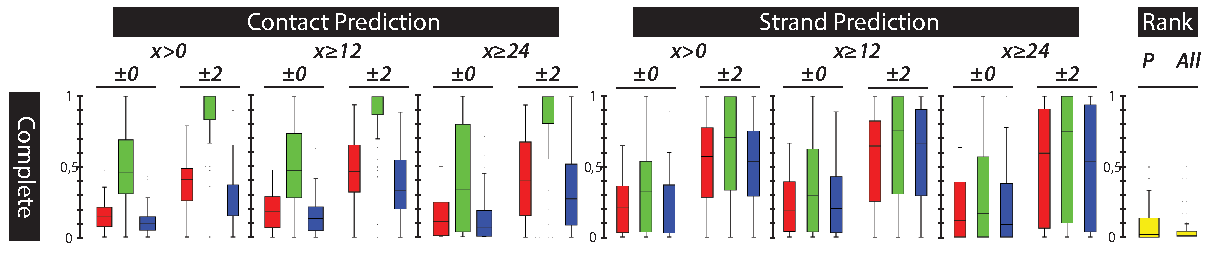
\includegraphics[scale=0.75, angle =0, clip=true, trim= 0 0 0 0]{Figs/BoxPlotComplete.pdf}
			\caption{ The performance of the proposed approach for contact prediction is evaluated based on the precision(green), recall(blue) and F-measure(red) of experimentally observed contacts. The performance metrics are reported for contacts which are 0, 12 and 24 residues apart. The metrics are also studied when predicted contacts are within $\pm 2$ residues of an observed contact.}  
		\label{fig:boxplots}
\end{figure}

\begin{figure}[H]
	 \centering
	 		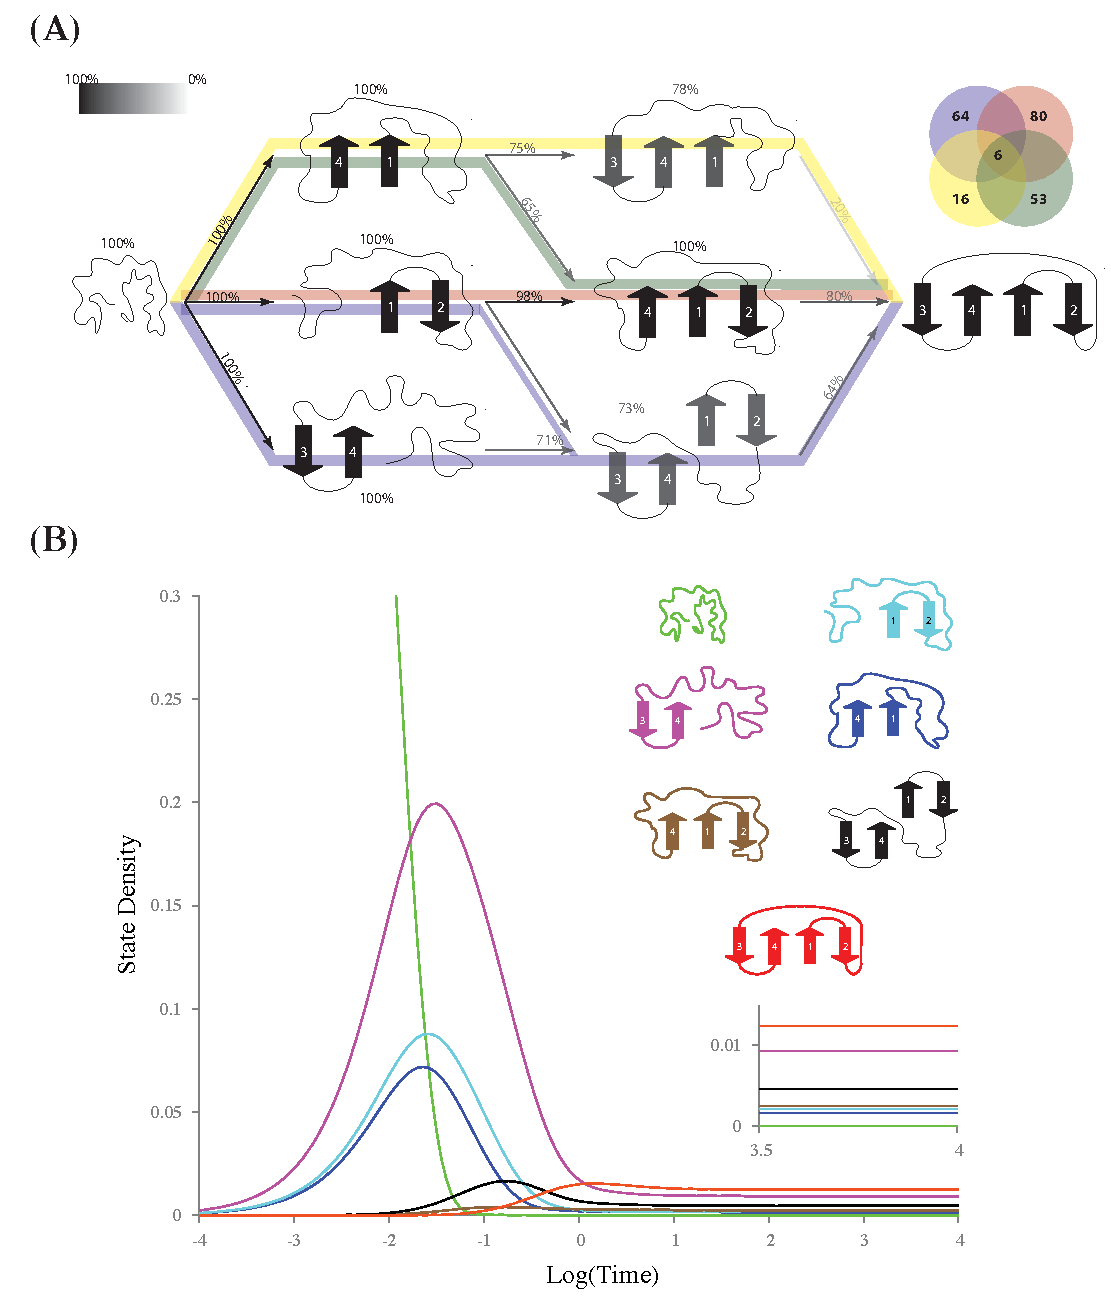
\includegraphics[scale=0.9, angle =0, clip=true, trim= 0 0 0 0]{Figs/1EM7.pdf}
			\caption{Pathways 1EM7: The figure represents the predicted transitions from a random coil to the native state of proteinG as a path in a graph of varyingly folded protein conformation states. The nodes in the graph represent energetically accessible conformation states which have been previously generated by the proposed Boltzmann-weighted ensemble sampling method. The percentage at top of each vertex (and its corresponding transparency) count for the number of times that this topology is predicted as a transition over the total number of runs. The vertices in the graph represent the transition between two topologies. The topologies connected by an edge are compatible topologies with structural similarity. The percentage at top of each edge (and its corresponding transparency) count for the number of times that this transition is found over the total number of runs. The predicted folding pathways are presented as paths in the graph. The percentage of presence of each path is presented through a Venn diagram at the right top corner of the figure. }  
		\label{fig:Pathways_1EM7}
\end{figure}

\begin{figure}[H]
	 \centering
	 		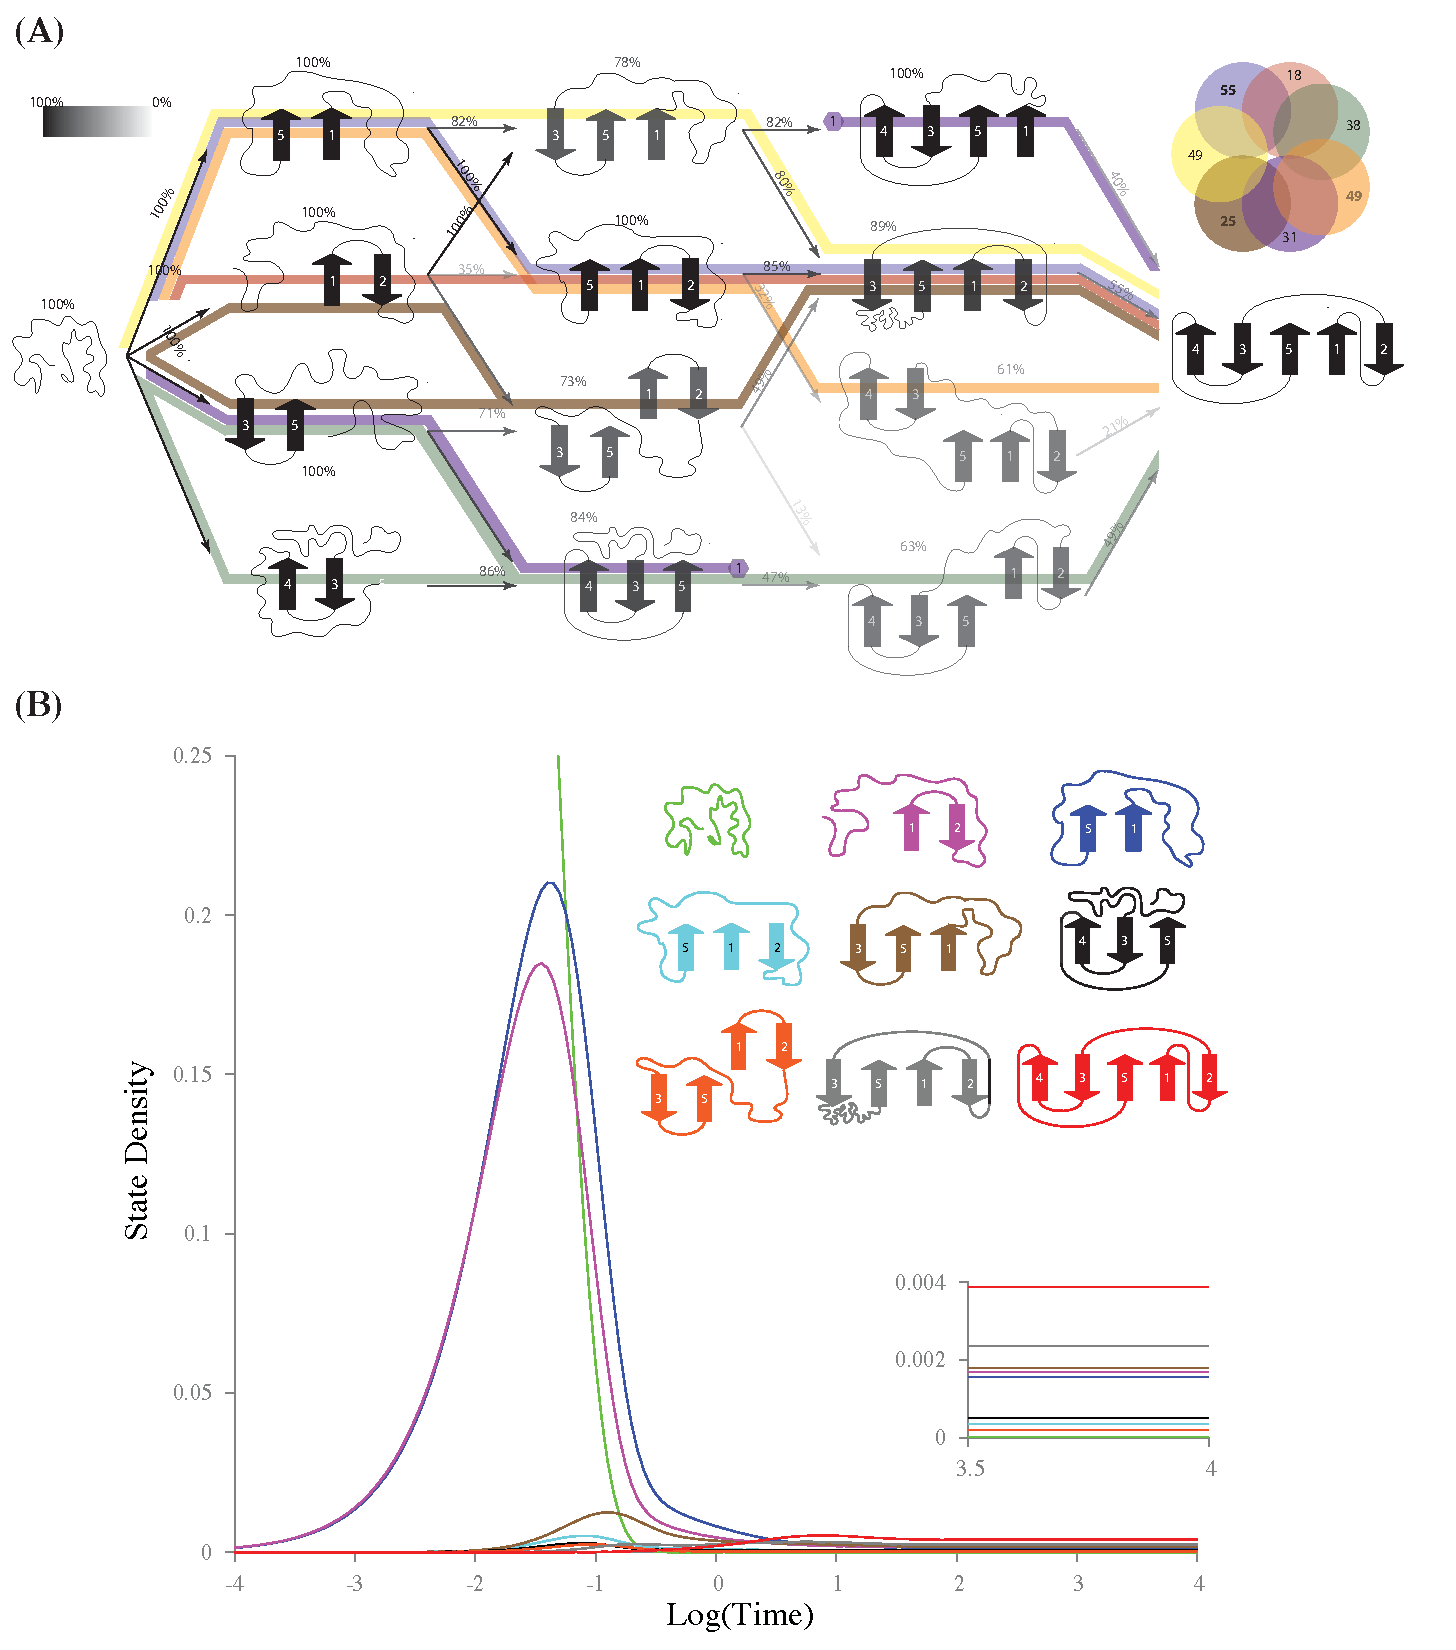
\includegraphics[scale=0.7, angle =0, clip=true, trim= 0 0 0 0]{Figs/1UBQ.pdf}
			\caption{Pathways 1EM7: The figure represents the predicted transitions from a random coil to the native state of proteinG as a path in a graph of varyingly folded protein conformation states. The nodes in the graph represent energetically accessible conformation states which have been previously generated by the proposed Boltzmann-weighted ensemble sampling method. The percentage at top of each vertex (and its corresponding transparency) count for the number of times that this topology is predicted as a transition over the total number of runs. The vertices in the graph represent the transition between two topologies. The topologies connected by an edge are compatible topologies with structural similarity. The percentage at top of each edge (and its corresponding transparency) count for the number of times that this transition is found over the total number of runs. The predicted folding pathways are presented as paths in the graph. The percentage of presence of each path is presented through a Venn diagram at the right top corner of the figure. }  
		\label{fig:Pathways_1EM7}
\end{figure}

\begin{figure}[H]
	 \centering
	 		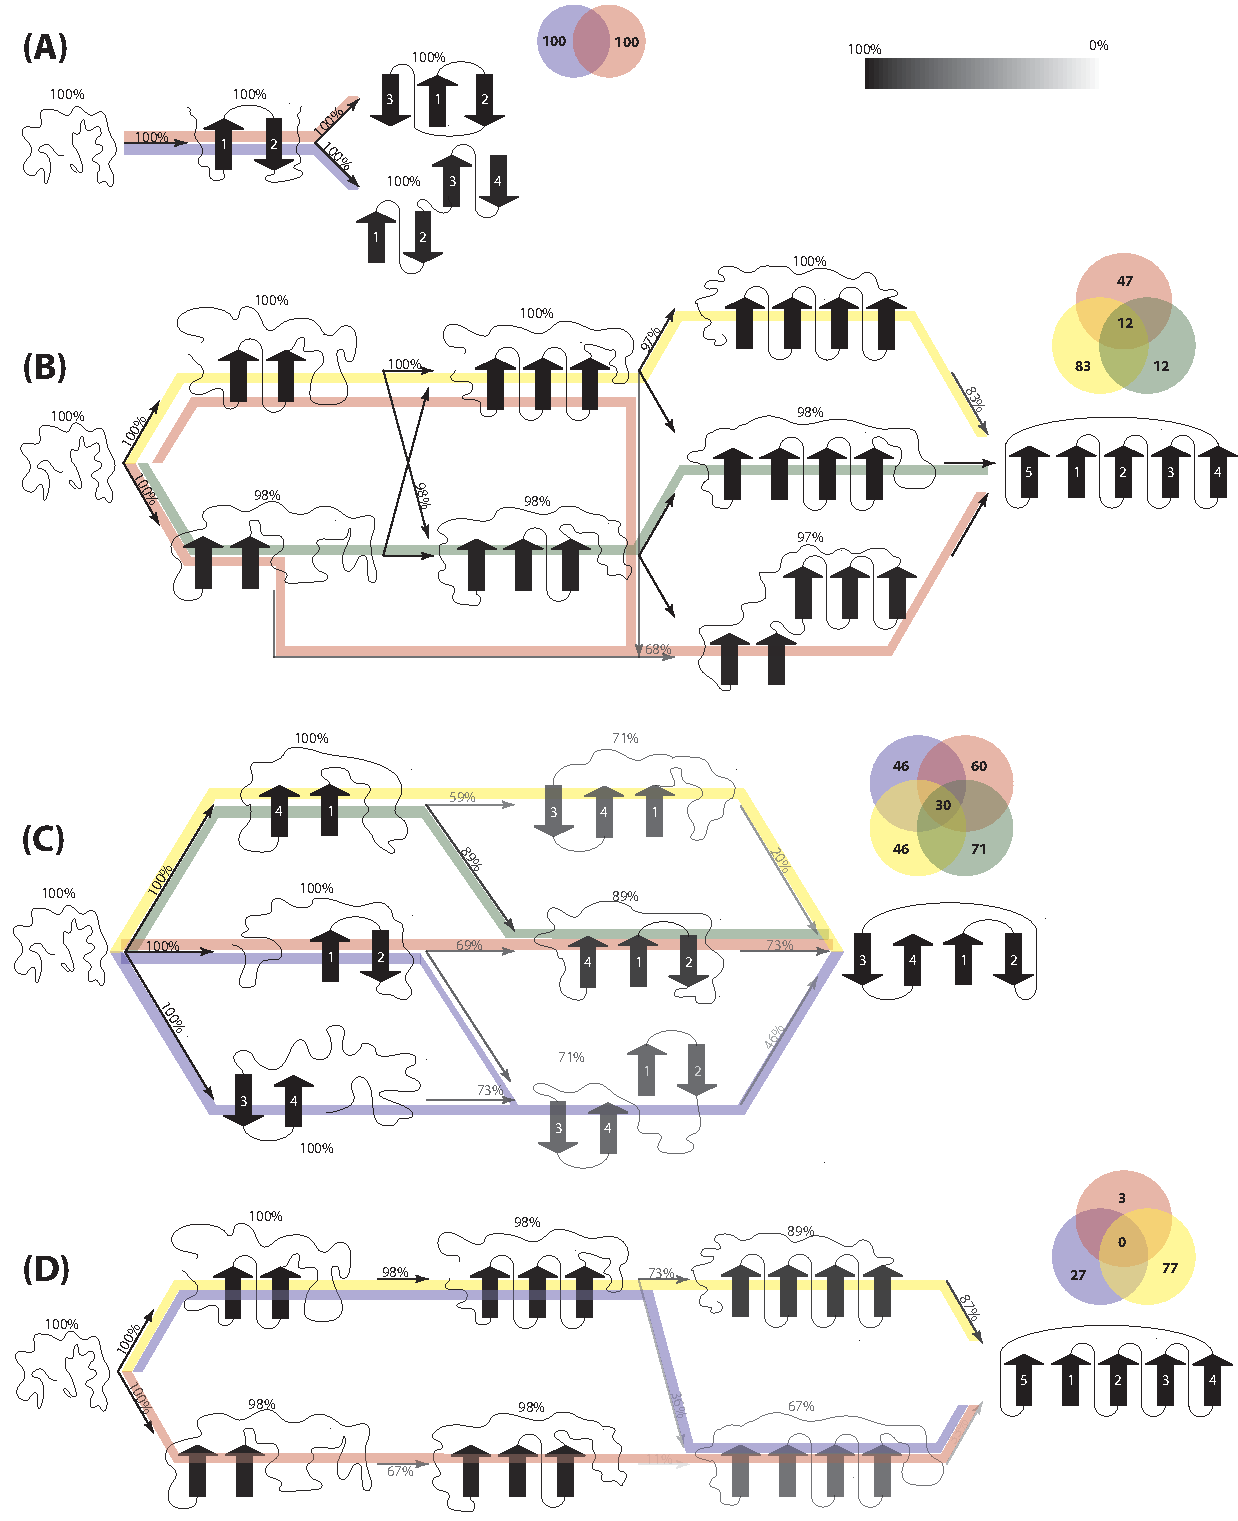
\includegraphics[scale=0.8, angle =0, clip=true, trim= 0 0 0 0]{Figs/Pfam.pdf}
			\caption{Pathways 1EM7: The figure represents the predicted transitions from a random coil to the native state of proteinG as a path in a graph of varyingly folded protein conformation states. The nodes in the graph represent energetically accessible conformation states which have been previously generated by the proposed Boltzmann-weighted ensemble sampling method. The percentage at top of each vertex (and its corresponding transparency) count for the number of times that this topology is predicted as a transition over the total number of runs. The vertices in the graph represent the transition between two topologies. The topologies connected by an edge are compatible topologies with structural similarity. The percentage at top of each edge (and its corresponding transparency) count for the number of times that this transition is found over the total number of runs. The predicted folding pathways are presented as paths in the graph. The percentage of presence of each path is presented through a Venn diagram at the right top corner of the figure. }  
		\label{fig:Pathways_1EM7}
\end{figure}

\begin{figure}[H]
	 \centering
	 		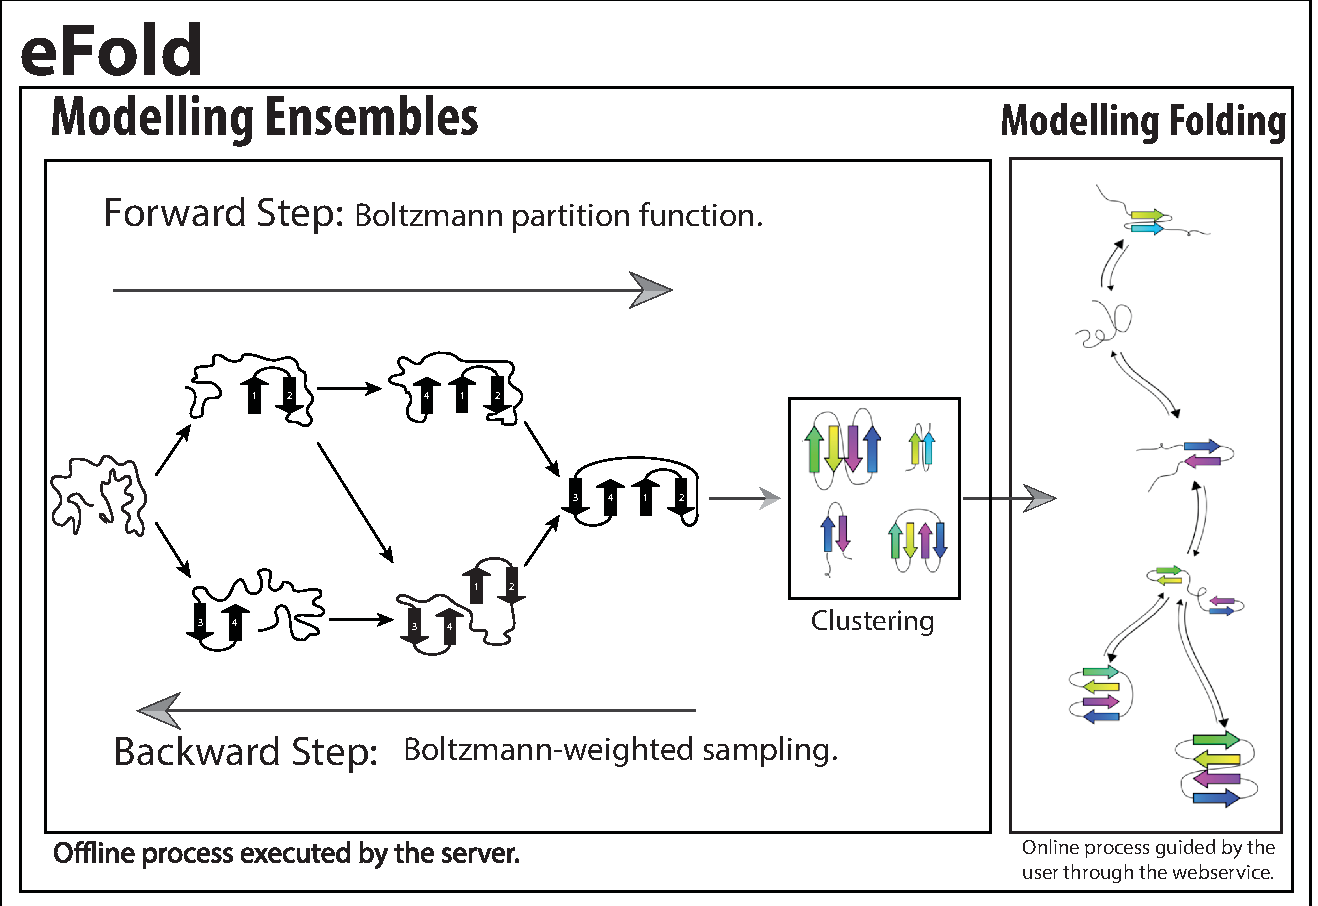
\includegraphics[scale=0.6, clip=true]{Figs/Method.pdf}
			\caption{\textbf{\texttt{efold}} is the proposed algorithm for predicting protein folding pathways and topologies using ensemble modelling and genomic variation. The algorithm is divided in two main phases, the modelling of ensembles and the modelling of the predicted folding dynamics. The first phase is computed off-line and it consist of a forward and backward traversal over the tree that model the hierarchical folding mechanism and that stores all the possible proteins states with its respective energies and likelihoods of occurrence. The second phase simulates the protein population dynamics based on the clusters computed in the previous phase. Specifically,  the transition from a random coil to the native state was modelled thorough a hierarchical assembly folding mechanism and it is represented as a path in a graph of varyingly folded protein conformation states. In this graph, the vertices are represented by energetically accessible conformation states presented in the clusters. The edges in the graph represent the possible folding pathways and the existence of structural similarity between the connected vertices. The user can change the structural similarity cutoff in order to generate different predicted protein pathways.}  
		\label{fig:method}
\end{figure}

\begin{figure}[H]
			\centering
	 		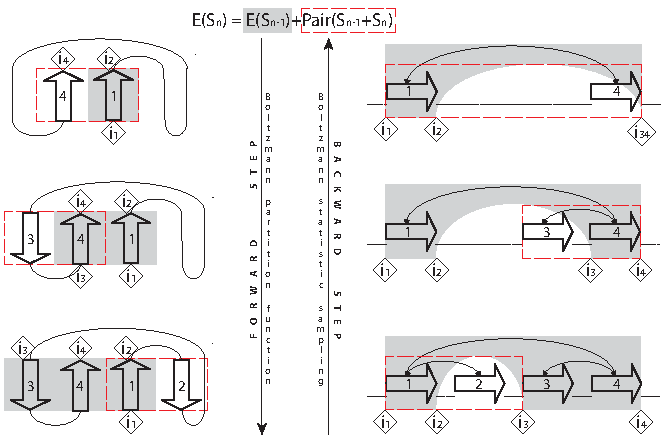
\includegraphics[scale=1.35, clip=true]{Figs/Topologies.pdf}
			\caption{\textbf{\texttt{efold} Topologies:} \textit{3A4P1A2} is the protein topology for the proteinG}  
		\label{fig:topologies}
\end{figure}







\section{Supplementary Materials}
\beginsupplement
\noindent \textbf{Supplementary Material} accompanies this paper at {\small {\tt http://http://csb.cs.mcgill.ca/efold/}}.


\begin{table}[H]
\footnotesize
\begin{center} {
\begin{tabular}{l| l*{10}{l}}
Protein & 1EM7 & $G_{B95}$ & $G_{A95}$ & $G_{B88}$ & $G_{A88}$  & $G_{B77}$ & $G_{A77}$ & $G_{B30}$ & $G_{A30}$ & $G_{B1}$ & $G_{A1}$ \\
\hline
1EM7 & 100 & 63 & 58 & 65 & 54 & 72 & 50 & 83 & 17 & 88 & 13 \\
$G_{B95}$ &  & 100 & 95 & 93 & 92 & 90 & 88 & 74 & 54 & 67 & 45  \\
$G_{A95}$ &  &  & 100 & 92 & 97 & 84 & 93 & 68 & 59 & 61 & 50  \\
$G_{B88}$ & &  &  & 100 & 88 & 93 & 84 & 77 & 50 & 70 & 42  \\
$G_{A88}$ &  &  &  &  & 100 & 81 & 97 & 65 & 63 & 58 & 54 \\
$G_{B77}$ &  &  &  &  &  & 100 & 77 & 84 & 43 & 77 & 34  \\
$G_{A77}$ &  &  &  &  &  &  & 100 & 61 & 67 & 54 & 58  \\
$G_{B30}$ &  &  &  &  &  &  &  & 100 & 31 & 93 & 24  \\
$G_{A30}$ &  &  &  &  &  &  &  &  & 100 & 24 & 92  \\
$G_{B1}$ &  &  &  &  &  &  &  &  &  & 100 & 17  \\
$G_{A1}$ &  &  &  &  &  &  &  &  &  &  & 100  \\
\end{tabular} }
\end{center}
\caption{\footnotesize Sequence identity between the different variants identified as $G_{A30}$, $G_{A77}$, $G_{A88}$, and $G_{A95}$ for the GA fold, and  $G_{B30}$, $G_{B77}$, $G_{B88}$, and $G_{B95}$ for the GB fold, and the wild type proteins $G_{A1}$ and $G_{B1}$ and the proteinG $1EM7$}
\label{tb:identity}
\end{table}

\begin{figure}[H]
	 \centering
	 		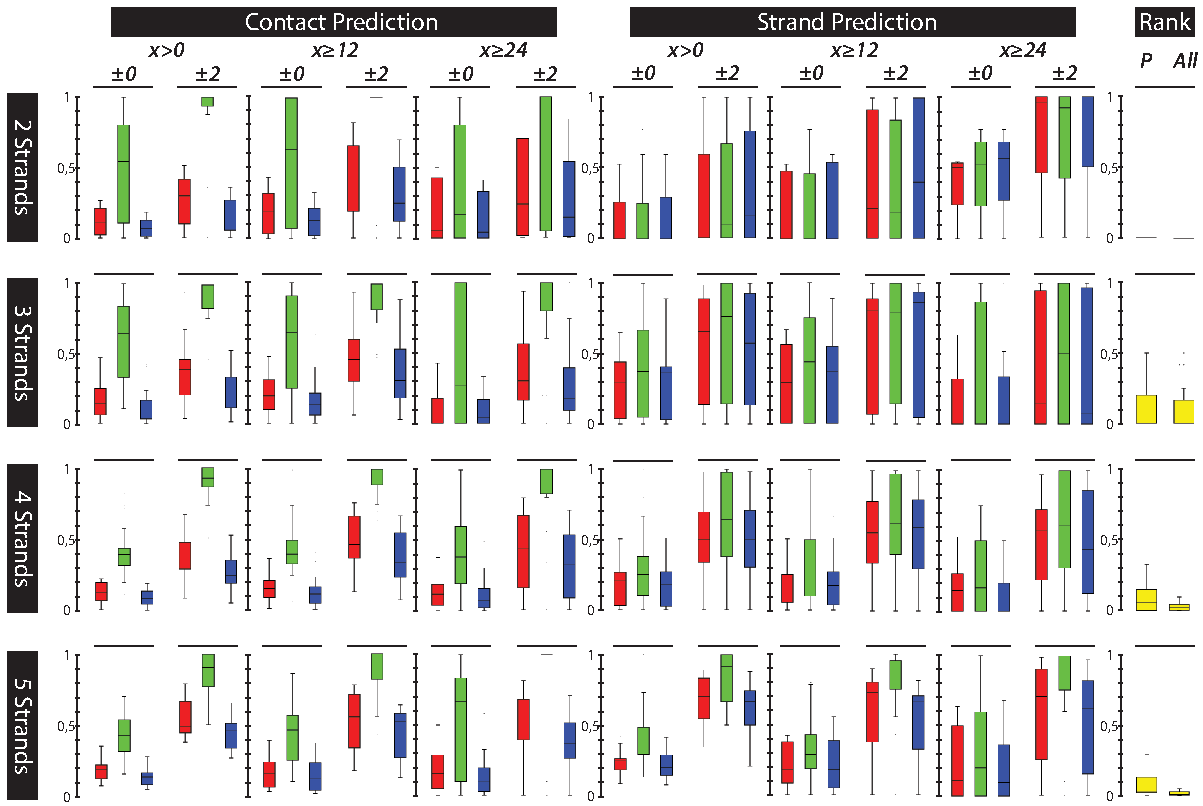
\includegraphics[scale=0.75, angle =0, clip=true, trim= 0 0 0 0]{Figs/BoxPlotsSplited.pdf}
			\caption{ The performance of the proposed approach for contact prediction is evaluated based on the precision(green), recall(blue) and F-measure(red) of experimentally observed contacts. The performance metrics are reported for contacts which are 0, 12 and 24 residues apart. The metrics are also studied when predicted contacts are within $\pm 2$ residues of an observed contact.}  
		\label{fig:boxplotSplited}
\end{figure}


\begin{figure}[H]
	 \centering
	 		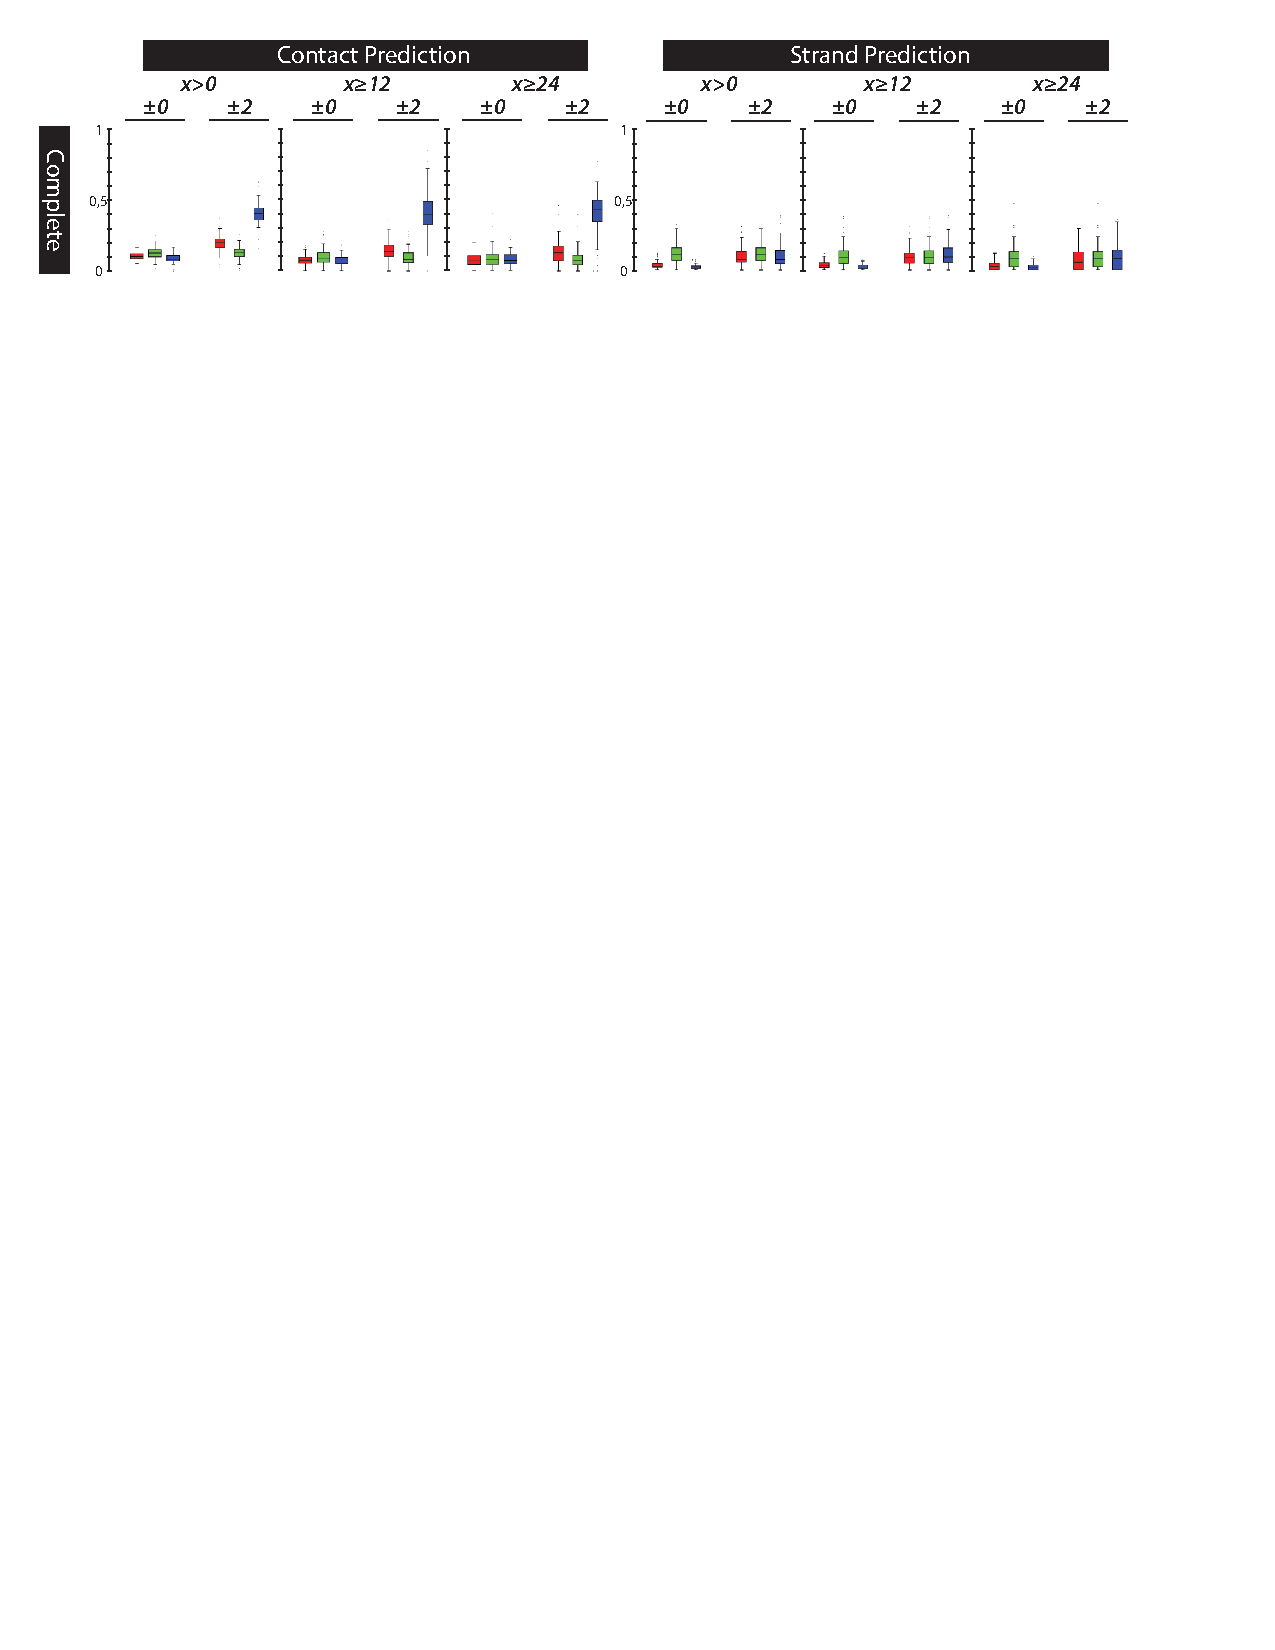
\includegraphics[scale=0.9, angle =0, clip=true, trim= 20 650 50 20]{Figs/BoxPlotsEvFold.pdf}
			\caption{ The performance of evfold for contact prediction is evaluated based on the precision(green), recall(blue) and F-measure(red) of experimentally observed contacts. The performance metrics are reported for contacts which are 0, 12 and 24 residues apart. The metrics are also studied when predicted contacts are within $\pm 2$ residues of an observed contact.}  
		\label{fig:boxplotsevfold}
\end{figure}



\bibliography{SAEfold}
\bibliographystyle{ScienceAdvances}


\noindent \textbf{Acknowledgements:} 
% Acknowledgments should be gathered into a paragraph after the final numbered reference. This section should also include 
% * complete funding information, 
% * a description of each author�s contribution to the paper, 
% * a listing of any competing interests of any of the authors (all authors must also fill out the Conflict of Interest form), and, 
% * a section on data and materials availability, information about the location of the data if not included in the paper, including **accession numbers** to any data relating to the paper and deposited in a public database.
%
The authors thank TBD for helpful conversations.\\
\noindent \textbf{Funding:} DB is supported by Colciencia's Francisco Jose de Caldas scholarship\\
\noindent \textbf{Author Contributions:} TBD\\
\noindent \textbf{Competing Interests:} The authors declare that they have no competing financial interests.\\
\noindent \textbf{Data and materials availability:} The \texttt{efold} web service, additional data and materials are available online at {\small {\tt http://csb.cs.mcgill.ca/efold/}}.










\end{document}




















